\chapter[Tècniques de TA]{Tècniques de traducció automàtica}
\label{se:TdTA}

\com{Ací faltaria parlar, en algun lloc, de la relació entre les
  arquitectures de traducció automàtica i el \emph{principi de
    composicionalitat}: treball per a Mikel, que ja té coses escrites.
  També caldria parlar (ací o en el tema d'ambigüitat) de la
  impossibilitat de programar el coneixement intuïtiu dels
  professionals de la traducció (creences, expectatives) per a desfer
  l'ambigüitat, generar text. etc. i de la necessitat de formular
  regles i mètodes per a automatitzar el procés. Tinc notes abundants
  i textos sobre això; el problema és on els col·loquem sense refer
  completament el tema.}

\com{Crec que es podria explicar el model zero i col·locar la
  \emph{traducció directa} com un cas típic de traducció indirecta
  \emph{ad hoc}}

Aquest capítol descriu les tècniques o, dit d'una altra manera, les
estratègies bàsiques usades pels programes de traducció automàtica.

Hi ha dos grans grups de sistemes de traducció automàtica:
\begin{itemize}
\item D'una banda, els sistemes de traducció automàtica \textbf{basats
    en regles} (en anglés, \emph{rule-based machine translation}) o
  \textbf{basats en coneixement} (en anglés \emph{knowledge-based
    machine translation}). En aquests sistemes, la informació
  necessària per a realitzar la traducció automàtica (diccionaris,
  regles) l'han escrita persones expertes de manera \emph{deductiva}:
  és a dir, han pensat en com automatitzar el procés de traducció
  automàtica i n'han deduït la informació necessària per a
  realitzar-la. Entre aquests sistemes, podem distingir:
  \begin{itemize}
  \item Els sistemes de traducció automàtica \emph{indirecta per
      transferència} (apartat~\ref{ss:classtrans}), entre els quals,
    podem distingir, d'acord amb el nivell d'abstracció lingüística:
    \begin{itemize}
    \item els sistemes de transferència morfològica avançada (de
      vegades anomenats de ``traducció directa'', tot i que no ho són;
      apartat~\ref{s3:STMorf});
    \item els sistemes de transferència sintàctica
      (apartat~\ref{s3:transyn}), i
    \item els sistemes de transferència semàntica
      (apartat~\ref{s3:transsem}).
    \end{itemize}
  \item Els sistemes de traducció automàtica \emph{per interlingua}
    (apartat~\ref{ss:interlingua}).
  \end{itemize}
\item D'altra banda, els sistemes de traducció automàtica
  \textbf{basats en corpus} (en anglés \emph{corpus-based machine
    translation}). En aquests sistemes (vegeu
  l'apartat~\ref{ss:induc}), la informació necessària per a realitzar
  la traducció automàtica s'\emph{aprén} automàticament de manera
  \emph{inductiva} a partir d'un \emph{corpus} paral·lel, és a dir, de
  grans quantitats de textos i les seues traduccions, prèviament
  \emph{segmentats} i \emph{alineats} per posar cada oració d'un text
  en correspondència amb la seua traducció en l'altre.\footnote{Els
    textos del corpus d'aprenentatge poden a més ser anotats o
    processats amb algun tipus de processador lingüístic com ara un
    analitzador morfològic o sintàctic.} Els sistemes basats en corpus
  més comuns són els de \emph{traducció automàtica estadística}, on el
  que s'aprenen són models probabilístics de traducció. Durant el
  decenni de 2010 s'està investigant en sistemes que usen l'anomenat
  \emph{aprenentatge profund} (en anglés \emph{deep learning}) basat
  en \emph{xarxes neurals artificials}, les quals es basen vagament en
  com funciona el cervell humà. 
\end{itemize}


%\section{La traducció automàtica basada en regles, entre el principi
%  de composicionalitat semàntica i la traducció mot per mot}
\section{Funcionament de la traducció automàtica}
\label{se:aprox}

Els sistemes de traducció automàtica \emph{reals}, és a dir, els que
s'usen en la realitat, són el resultat de fer una series
d'aproximacions sobre la traducció automàtica \emph{ideal} per fer el
problema de la traducció computacionalment abordable.

La majoria dels sistemes de traducció automàtica, independentment de
si són basats en regles o en corpus, adopten la que podrien anomenar
\textbf{aproximació oracional}, segons la qual \emph{traduir texts és
  traduir oracions}. Aquesta aproximació exclou el tractament d'alguns
aspectes de l'estructura del discurs.

Una vegada feta aquesta aproximació general, la resta d'aproximacions
depenen del tipus de sistema de traducció automàtica. La majoria dels
sistemes de traducció automàtica basats en coneixement aborden la
traducció com l'aplicació del \emph{principi de composicionalitat
  semàntica} (PCS, capítol~\ref{se:ambig}), el qual afirma que la
interpretació (el significat) d'una oració es construeix
composicionalment a partir de les interpretacions dels mots, seguint
els agrupaments dictats pel seu arbre d'anàlisi sintàctica, i també al
revés, que les oracions es poden construir composicionalment a partir
de les interpretacions \citep{tellier00p}. Traduir una oració, en
aquest esquema, comporta:
\begin{itemize}
\item fer-ne l'anàlisi sintàctica completa,
\item assignar interpretació a cada mot,
\item construir composicionalment una interpretació de l'oració,
\item analitzar-la per a obtenir mots i un arbre d'anàlisi sintàctica
  per a la llengua meta (LM), i
\item generar una oració en LM a partir dels mots i l'arbre.
\end{itemize}
Aquest és bàsicament el \emph{modus operandi} dels sistemes
d'\emph{interlingua} (que es discutiran en la
secció~\ref{ss:interlingua}) i constitueix l'\textbf{aproximació
  composicional}. No oblidem que aquesta descripció assumeix que
l'ambigüitat lèxica (múltiples interpretacions dels mots) i
estructural (més d'un arbre d'anàlisi sintàctica) ha estat idealment
resolta.

D'una altra part, els sistemes de traducció automàtica indirecta per
transferència (que es discutiran en l'apartat \ref{ss:classtrans}) són
el resultat d'una sèrie d'aproximacions (moltes d'elles inevitables)
sobre un model ideal i teòricament motivat basat en el \emph{principi
  de composicionalitat semàntica}. Aquests sistemes també es poden veure
com el resultat d'una sèrie de refinaments inevitables sobre un
sistema de traducció \emph{mot per mot} (vegeu
l'apartat~\ref{ss:dirindir}), és a dir, com una sèrie d'operacions
addicionals que s'han de fer a més d'anar substituint cada mot per un
equivalent constant. Per exemple, per a produir traduccions
acceptables, ràpides i intel·ligibles, fins i tot entre llengües molt
semblants, s'ha d'afegir un processament lèxic robust (per exemple,
per a tractar expressions multimot o per a elegir equivalents adequats
per a mots lèxicament ambigus) i un processament estructural local o
global que es basa en regles simples i ben formulades per a algunes
transformacions estructurals (reordenaments, concordança,
etc.). 

% Aquests refinaments impliquen necessàriament un cert nivell
% d'anàlisi del text original, el qual produeix una representació
% intermèdia, abstracta, d'aquest: el sistema de traducció automàtica
% esdevé \emph{indirecte}, com ara els sistemes de transferència
% discutits amb més detall més avall (apartat~\ref{ss:classtrans}).

Com en el cas dels traductors professionals, els sistemes de traducció
automàtica no sempre necessiten \emph{comprendre} les frases en
llengua origen (LO) , és a dir, construir-ne una interpretació
explícita. Aquesta noció, que pot semblar polèmica, no ho és tant: qui
tradueix com a professional un manual de mecànica de l'automòbil o un
text de física teòrica ho pot fer sense haver d'entendre completament
les disciplines corresponents. Els sistemes de \emph{transferència}
sintàctica (vegeu l'apartat \ref{s3:transyn}) prenen una drecera i van
directament de l'arbre d'anàlisi sintàctica i els mots en LO a l'arbre
i els mots en LM. Ho fan aplicant transformacions a l'arbre d'anàlisi
sintàctica (\emph{transferència estructural}) i substituint els mots
(\emph{transferència lèxica}), sense construir una representació
explícita de la interpretació; aquesta és l'\textbf{aproximació de
  transferència}. Depenent del tipus concret de sistema de traducció
automàtica per transferència, encara són possibles més aproximacions,
com veurem més avall.

% \item[Aproximació núm.\ 3:] Quan les llengües involucrades són
%   sintàcticament similars (per exemple, quan estan emparentades),
%   no es fa l'anàlisi sintàctica completa: la transferència lèxica
%   és completa però la transferència estructural és parcial i local
%   i només es fa on és necessària.  Aquesta aproximació és
%   l'aproximació de la \emph{transferència parcial}. Els sistemes
%   anomenats \emph{transformers} o també de transferència
%   morfològica
%   avançada (vegeu~\ref{s3:STMorf}) \citep[4.2]{arnold94b}, molts
%   dels quals estan disponibles per Internet,\footnote{Per exemple,
%   SDL Transcend està disponible en
%   \url{http://www.freetranslation.com} i Reverso, en
%   \url{http://www.reverso.net}.} són exemples d'aquesta
%   aproximació.

Per últim, el sistemes de traducció automàtica estadística (que es
discutiran en l'apartat \ref{ss:induc}) fan \textbf{assumpcions
  d'independència estadística} per poder modelar estadísticament el
procés de traducció. Per exemple, el \emph{model de traducció}, que
s'usa per estimar la probabilitat de què un segment de text en LM siga
la traducció d'un segment de text en LO, assumeix que la traducció
d'un segment és independent de la traducció de la resta de segments de
l'oració; és a dir, assumeix que no cal tenir en compte el context per
a traduir cadascun dels segments de l'oració en LO.

\section{Traducció directa i traducció indirecta}
\label{ss:dirindir} 
Les estratègies de traducció automàtica es poden dividir en dos grans
grups, les \emph{directes} i les \emph{indirectes}. L'estratègia
\emph{directa} s'anomena així perquè la traducció d'una frase es
produeix directament, sense que es genere una representació intermèdia
de la frase; de vegades també se sol anomenar vagament traducció
\emph{mot per mot}. L'estratègia \emph{indirecta} produeix, a partir
de la frase en LO, una representació intermèdia de la frase que
després s'usa per a traduir-la. Veurem més endavant de quina
naturalesa són aquestes representacions intermèdies.

\label{pg:mpm}
Una formalització possible de la traducció automàtica directa més
senzilla possible és la traducció \emph{mot a mot}: el sistema llig el
text original mot a mot d'esquerra a dreta,\footnote{S'assumeix que el
  text està ja segmentat en mots, operació que pot no ser trivial en
  alguns idiomes com ara el japonés o el xinès, que no usen espais en
  blanc per a separar els mots.} substitueix cada mot original per un
equivalent fix (d'un mot, de més mots, o fins i tot de zero mots) en
LM sense tenir en compte el context i escriu els mots un a un i en el
mateix ordre en el text meta.  Per exemple, si la frase té \(N\) mots,
\begin{displaymath}
  m_1\; m_2\; m_3\; \cdots \;m_N
\end{displaymath}
la traducció \emph{mot per mot} és
\begin{displaymath}
  T(m_1)\; T(m_2)\; T(m_3)\; \cdots\; T(m_N)
\end{displaymath}
on \(T(m)\) representa l'equivalent fix del mot \(m\) en la LM, que
pot tenir zero, un o més mots. Per exemple, la traducció \emph{mot per
  mot} a l'anglés de la frase catalana \emph{Aquest exercici pràctic
  és molt senzill}, amb \(m_1=\mbox{\emph{Aquest}}\),
\(m_2=\mbox{\emph{exercici}}\), etc., podria ser \emph{This exercise
  practical it is very simple} (incorrecta), on, per exemple,
\(T(m_4)=T(\mbox{\emph{és}})=\mbox{\emph{it is}}\).

Cap sistema real de traducció automàtica usa aquest model tan
rudimentari de traducció, ja que és incapaç de produir traduccions
automàtiques útils, ni tan sols per a llengües molt similars: tots els
sistemes van més enllà i realitzen operacions addicionals. Per això
mateix, el model \emph{mot a mot} es pot usar com a model de
referència o \emph{model zero} a l'hora d'estudiar què més fan els
sistemes existents, o què més cal fer per a produir traduccions
automàtiques útils per a un parell de llengües.

% Una aproximació a la traducció humana assistida per ordinador (és a
% dir, semiautomàtica) que es pot veure com un tipus de traducció
% directa ---que usa segments de text més llargs com ara les oracions
% en compte dels mots--- és la que s'usa en les anomenades
% \emph{memòries de traducció} (vegeu el capítol~\ref{se:memtrad}).
 
\section{Traducció indirecta per transferència}
\label{ss:classtrans}

Molts dels sistemes indirectes basats en regles són sistemes de
\emph{transferència}. Un \emph{sistema de traducció automàtica
  indirecta per transferència}, o, abreviadament, \emph{sistema de
  transferència} és el que fa les traduccions en tres fases ben
diferenciades anomenades \emph{anàlisi}, \emph{transferència} i
\emph{generació}; cada una d'aquestes fases és realitzada per un mòdul
(un subprograma) del sistema:
\begin{itemize}
\item El mòdul d'\emph{anàlisi} és un mòdul monolingüe que produeix, a
  partir de la frase en LO, una \emph{representació abstracta del text
    origen} (RATO). En la RATO s'eliminen tots els detalls de la frase
  en LO que no es consideren rellevants per a la traducció i se'n
  destaquen aquelles característiques i relacions que sí que ho són.
  Per exemple, podria convenir que les frases angleses ``Sam gave a
  book to Leslie'' i ``Sam gave Leslie a book'' \citep{arnold93j}
  tingueren la mateixa RATO.
\item El mòdul de \emph{transferència} és un mòdul bilingüe que llig
  la RATO i genera una altra representació abstracta similar, però per
  a la LM, la \emph{representació abstracta del text meta} (RATM).
\item El mòdul de \emph{generació} (o, menys comunament,
  \emph{síntesi}) genera a partir de la RATM un text \emph{concret}:
  la traducció en brut.
\end{itemize}
Aquestes tres fases s'esquematitzen en la figura~\ref{fg:transfer}.


\begin{figure}
\begin{center}
\parbox{0.5cm}{TO} $\to$
\framebox{\parbox{0.2cm}{A}} $\to$ 
\parbox{1.0cm}{RATO} $\to$
\framebox{\parbox{0.2cm}{T}} $\to$
\parbox{1.25cm}{RATM} $\to$
\framebox{\parbox{0.25cm}{G}} $\to$
\parbox{0.5cm}{TM} 
\end{center}
\caption{Fases d'anàlisi (A), transferència (T) i generació (G) en un
  sistema de traducció indirecta per transferència (TO = text origen;
  RATO = representació abstracta del text origen; RATM = representació
  abstracta del text meta; TM = text meta).}
\label{fg:transfer} 
\end{figure}

Les representacions abstractes \emph{apropen} les dues llengües
eliminant-ne alguns detalls específics i destacant característiques
generals que poden així ser tractades més fàcilment pel mòdul de
transferència. Per exemple, els adjectius catalans van normalment
darrere dels substantius mentre que els anglesos van normalment
davant; traduir comporta, per tant, canviar els adjectius de
posició. Però per a això, cal identificar quines paraules són
adjectius i substantius: la fase d'anàlisi es pot encarregar d'aquesta
tasca perquè la fase de transferència puga aplicar regles generals
sense preocupar-se de quins són els adjectius o els substantius
concrets.

% \begin{figure} % figura vella
% \begin{center}
% %TexCad Options
% %\grade{\off}
% %\emlines{\off}
% %\beziermacro{\on}
% %\reduce{\on}
% %\snapping{\off}
% %\quality{2.00}
% %\graddiff{0.01}
% %\snapasp{1}
% %\zoom{1.00}
% \unitlength 1.00mm
% \linethickness{0.4pt}
% \begin{picture}(100.00,20.00)
% \put(10.00,10.00){\makebox(0,0)[cc]{text LO}}
% \put(40.00,10.00){\makebox(0,0)[cc]{RALO}}
% \put(70.00,10.00){\makebox(0,0)[cc]{RALM}}
% \put(100.00,10.00){\makebox(0,0)[cc]{text LM}}
% %\vector(20.00,10.00)(30.00,10.00)
% \put(30.00,10.00){\vector(1,0){0.2}}
% \put(20.00,10.00){\line(1,0){10.00}}
% %\end
% %\vector(50.00,10.00)(60.00,10.00)
% \put(60.00,10.00){\vector(1,0){0.2}}
% \put(50.00,10.00){\line(1,0){10.00}}
% %\end
% %\vector(80.00,10.00)(90.00,10.00)
% \put(90.00,10.00){\vector(1,0){0.2}}
% \put(80.00,10.00){\line(1,0){10.00}}
% %\end
% \put(25.00,15.00){\makebox(0,0)[cc]{anàl.}}
% \put(55.00,15.00){\makebox(0,0)[cc]{transf.}}
% \put(85.00,15.00){\makebox(0,0)[cc]{gen.}}
% \end{picture}
% \end{center}
% \caption{Fases d'anàlisi, transferència i generació en un
% sistema de traducció indirecta per transferència.}
% \label{fg:transfer} 
% \end{figure}

L'arquitectura de transferència és el model estàndard per a la
traducció automàtica basada en regles o coneixement contemporània, i
ho ha estat per molts anys \citep{arnold93j}.

Els sistemes de transferència es classifiquen segons la naturalesa de
les representacions abstractes que utilitzen: es pot parlar, en ordre
de profunditat de l'anàlisi, de sistemes de \emph{transferència
  morfològica}, de \emph{transferència sintàctica} o de {\em
  transferència semàntica}.  L'elecció de la profunditat de l'anàlisi
s'ha de fonamentar en la naturalesa i la profunditat de les
divergències de traducció \citep{vandooren93b} entre les llengües
implicades.

L'arquitectura de transferència té tres característiques interessants
que mereixen ser esmentades:
\begin{description}
\item[Funcionament com a cadena de muntatge.] El sistema de
  transferència funciona com una \emph{cadena de muntatge}: com que
  els tres mòduls treballen d'esquerra a dreta i en una única passada,
  no cal que un mòdul espere que l'anterior acabe amb el text: poden
  treballar paral·lelament; això fa que els sistemes d'aquesta
  naturalesa siguen molt ràpids.
\item[Modularitat.] La divisió en \emph{mòduls} o etapes ben
  diferenciades (anàlisi, transferència i generació) en permet la
  reutilització. Per exemple, si hem construït un sistema de
  transferència que tradueix de l'anglés a l'espanyol:
  \begin{center}
 \parbox{0.5cm}{en} $\to$
 \framebox{\parbox{0.5cm}{A\(_\mathrm{en}\)}} $\to$ 
 \framebox{\parbox{1.125cm}{T\(_\mathrm{en\to es}\)}} $\to$
 \framebox{\parbox{0.5cm}{G\(_\mathrm{es}\)}} $\to$
 \parbox{0.5cm}{es} 
 \end{center}
 podem aprofitar el mòdul d'anàlisi de l'anglés (A\(_\mathrm{en}\))
 per a construir un sistema de l'anglés al català:
 \begin{center}
 \parbox{0.5cm}{en} $\to$
 \framebox{\parbox{0.5cm}{A\(_\mathrm{en}\)}} $\to$ 
 \framebox{\parbox{1.125cm}{T\(_\mathrm{en\to ca}\)}} $\to$
 \framebox{\parbox{0.5cm}{G\(_\mathrm{ca}\)}} $\to$
 \parbox{0.5cm}{ca} 
 \end{center}
 o usar el mòdul de generació de l'espanyol G\(_\mathrm{es}\) per a
 construir un sistema del neerlandés a l'espanyol:
 \begin{center}
 \parbox{0.5cm}{en} $\to$
 \framebox{\parbox{0.5cm}{A\(_\mathrm{nl}\)}} $\to$ 
 \framebox{\parbox{1.125cm}{T\(_\mathrm{nl\to es}\)}} $\to$
 \framebox{\parbox{0.5cm}{G\(_\mathrm{es}\)}} $\to$
 \parbox{0.5cm}{es} 
 \end{center}
\item[Reversibilitat parcial.]  Si se separen les dades lingüístiques
  usades per cada un dels tres mòduls,\label{pg:separacio} és possible una
  \emph{reversibilitat parcial}.  Si en el sistema anglés--espanyol de
  dalt separem les \emph{dades lingüístiques} de cada un dels tres
  mòduls del \emph{programari} que processa aquestes dades
  (dA\(_\mathrm{en}\), dT\(_\mathrm{en\to es}\), dG\(_\mathrm{es}\))
  podem definir un \emph{motor} genèric de traducció (A, T, G) que val
  per a qualsevol parell de llengües:
 \begin{center}
 \parbox{0.5cm}{en} $\to$
\framebox{\parbox{0.75cm}{dA\(_\mathrm{en}\)\\ A}} $\to$
\framebox{\parbox{1.5cm}{dT\(_\mathrm{en\to es}\)\\ T}} $\to$
\framebox{\parbox{0.75cm}{dG\(_\mathrm{es}\)\\ G}} $\to$
 \parbox{0.5cm}{es}
\end{center} 
Si ara volem escriure el sistema de traducció invers,
espanyol--anglés, és a dir,
 \begin{center}
 \parbox{0.5cm}{es} $\to$
\framebox{\parbox{0.75cm}{dA\(_\mathrm{es}\)\\ A}} $\to$
\framebox{\parbox{1.5cm}{dT\(_\mathrm{es\to en}\)\\ T}} $\to$
\framebox{\parbox{0.75cm}{dG\(_\mathrm{en}\)\\ G}} $\to$
 \parbox{0.5cm}{en}
 \end{center} 
 podríem traure avantatge del fet que hi ha grans semblances entre les
 dades lingüístiques de aquest sistema i les del sistema anterior:
\begin{itemize}
\item les dades que necessitem per a l'anàlisi de l'espanyol
  dA\(_\mathrm{es}\) són molt similars a les dades de generació de
  l'espanyol dG\(_\mathrm{es}\) del sistema existent: per a analitzar
  l'espanyol podem reciclar una bona part de les dades que s'usaven
  per a generar-lo en el sistema anterior;
\item les dades que necessitem per a la generació de l'anglés
  dG\(_\mathrm{en}\) són molt similars a les dades d'anàlisi de
  l'anglés dA\(_\mathrm{en}\) del sistema existent: per a generar
  l'anglés podem reciclar una bona part de les dades que s'usaven per
  a analitzar-lo en el sistema anterior;
\item les dades de transferència de l'espanyol a l'anglés
  dT\(_\mathrm{es\to en}\) són molt similars a les dades de
  transferència de l'anglés a l'espanyol dT\(_\mathrm{en\to es}\) del
  sistema existent: per a transferir d'espanyol a anglés podem usar
  una bona part de les dades que s'usaven per a transferir des de
  l'anglés a l'espanyol en el sistema anterior (per exemple, podem
  ``pegar la volta'' als diccionaris bilingües i podríem aprofitar-ne
  moltes entrades).
\end{itemize}
\end{description}

\subsection{Sistemes de transferència morfològica avançada}
\label{s3:STMorf}

En els sistemes de \emph{transferència morfològica avançada} ---també
anomenats sistemes de \emph{transferència sintàctica parcial} o
\emph{transformers} \citep[4.2]{arnold94b}--- la fase d'\emph{anàlisi}
analitza morfològicament els mots de la frase i els desambigua en cas
d'ambigüitat lèxica categorial però només identifica les relacions
(sintàctiques) entre ells usant patrons molt senzills.\footnote{Alguns
  sistemes de transferència morfològica avançada disponibles en
  Internet són: SDL Transcend (\url{http://www.freetranslation.com})
  Reverso (\url{http://www.reverso.net}), i Apertium
  (\url{http://www.apertium.org}).}  La secció~\ref{s3:anmor} dóna més
detalls sobre els processos i els mètodes d'anàlisi i generació
morfològiques.

De fet, els sistemes de transferència morfològica avançada es poden
veure com el resultat de fer una tercera aproximació, afegida a les
dues (\emph{aproximació oracional} i \emph{aproximació de
  transferència}) discutides en l'apartat~\ref{se:aprox}:
\begin{quote}
  \textbf{Aproximació de transferència parcial:} Quan les llengües
  involucrades no són massa diferents sintàcticament (per exemple,
  quan estan emparentades), no cal fer l'anàlisi sintàctica completa:
  la transferència lèxica és completa però la transferència
  estructural és parcial i local i només es fa on és necessària.
\end{quote}

La fase de \emph{transferència} pot consistir en un reordenament local
(\emph{transferència estructural}) d'algunes seqüències de mots (per
exemple, quan es tradueix de l'anglés al català, els parells
adjectiu--substantiu es podrien reordenar a substantiu--adjectiu) i en
la conversió de les formes lèxiques de la LO en les corresponents de
la LM mitjançant l'ús d'un diccionari bilingüe (\emph{transferència
  lèxica}).

La fase de \emph{generació} podria efectuar la substitució de les
formes lèxiques de la LM per les corresponents formes superficials.

Com que els sistemes de transferència morfològica avançada no
identifiquen realment les relacions sintàctiques entre els mots de la
frase en la llengua d'origen, per a fer els reordenaments han
d'identificar les seqüències de mots que necessiten ser reordenats. La
capacitat d'un sistema de transferència morfològica per a produir
traduccions acceptables dependrà de la seua capacitat per a detectar
seqüències de mots que es corresponguen amb els sintagmes que
necessiten ser reordenats.  Imaginem que volem traduir de l'anglés al
català i hem decidit que s'han d'usar aquestes regles de reordenament:
\begin{itemize}
\item [$R_1$] (en) \textbf{adj} \textbf{subst} $\rightarrow$ (ca)
  \textbf{subst} \textbf{adj}
\item [$R_2$] (en) \textbf{subst}$_1$ \textbf{subst}$_2$ $\rightarrow$
  (ca) \textbf{subst}$_2$ \textbf{prep\_de} \textbf{subst}$_1$
\end{itemize}
Per exemple, la regla $R_1$ reordenaria ``tall driver'' en
``conductor alt'' i la regla $R_2$ reordenaria ``truck driver''
en ``conductor de camió''. 

Ara, pensem què li succeiria a ``tall truck driver''. Si s'aplica
primer la regla $R_1$ a ``tall truck'' ja no podem aplicar-hi la
$R_2$. Si s'hi aplica primer la $R_2$ i després la $R_1$, s'obté la
traducció correcta: ``conductor alt de camió''. Quan tenim més d'una
regla, no sabem en quin ordre cal aplicar-les-hi. Si tenim ``tall
gasoline truck driver'' (``conductor alt de camió de gasolina''), no
hi ha cap ordre d'aplicació de $R_2$ i $R_1$ que done una traducció
acceptable.  Això suggereix la necessitat d'una nova regla que detecte
i reordene el patró llarg
adjectiu--substantiu--substantiu--substantiu, per exemple:
\begin{itemize}
\item[$R_3$] (en) \textbf{adj} \textbf{subst}$_1$ \textbf{subst}$_2$ \textbf{subst}$_3$
$\rightarrow$ (ca) \textbf{subst}$_3$ \textbf{adj} \textbf{prep\_de} \textbf{subst}$_2$ \textbf{prep\_de} \textbf{subst}$_1$
\end{itemize}  
Aquesta regla podria reordenar correctament aquesta seqüència de
quatre mots. Com es pot veure, les regles de reordenament intenten
descobrir unitats sintàctiques (sintagmes) usant un nombre limitat de
patrons que representen les seqüències de mots que poden formar
aquestes unitats; el problema és que els sintagmes poden ser, en
principi, indefinidament llargs,\footnote{En la gramàtica de la
  llengua, si una regla que estén un sintagma es pot aplicar
  repetidament a un determinat tipus de sintagma, aquest sintagma es
  pot allargar indefinidament. Un exemple clàssic d'això el donen les
  oracions adjectives de relatiu; la sèrie de sintagmes nominals ``el
  cotxe'', ``el cotxe que va dur l'home'', ``el cotxe que va dur
  l'home que va vindre del poble'', ``el cotxe que va dur l'home que
  va vindre del poble que vam visitar durant el viatge'', etc.,
  demostra que no hi ha límits a la longitud d'un sintagma (nominal,
  en aquest cas).} i el conjunt de regles de reordenament ha de ser
forçosament limitat.

Queda, a més, per determinar, en els casos en què es pot aplicar més
d'una regla, quina s'hi ha d'aplicar abans; en una oració llarga i amb
moltes regles disponibles, açò pot ser un problema greu. Una tècnica
observada en alguns programes és la següent: (a) els reordenaments es
van aplicant segons es recorre la frase d'esquerra a dreta; (b) els
reordenaments de seqüències més llargues tenen prioritat, i (c) els
mots afectats per un reordenament no tornen a estar involucrats en cap
altre reordenament. Així només es visita una vegada cada mot de la
frase. Si no es pot aplicar un reordenament al primer mot pendent de
processar, es tradueix aïlladament i es continua amb el següent mot.

Per a poder traduir \emph{tall truck driver} seguint aquest esquema,
caldria una regla que combinara \(R_1\) i \(R_2\):
\begin{itemize}
\item[$R_4$] (en) \textbf{adj} \textbf{subst}$_1$ \textbf{subst}$_2$ 
$\rightarrow$ (ca) \textbf{subst}$_2$ \textbf{adj} \textbf{prep\_de} \textbf{subst}$_1$ 
\end{itemize}  


La identificació de patrons de categories morfològiques que es
corresponguen amb els sintagmes més freqüents pot servir, a més de per
a fer reordenaments, per a resoldre la concordança de nombre i
gènere. Per exemple, si usem el patró substantiu--adjectiu per a
identificar una classe de sintagmes nominals senzills, podem fer que
la traducció correcta al català del sintagma nominal espanyol {\em
  postre buenísimo} siga \emph{postres boníssimes}, ja que el gènere i
el nombre de l'adjectiu que modifica a un substantiu ha de
concordar-hi i el substantiu espanyol \emph{postre} (masculí singular)
es correspon amb el substantiu català \emph{postres} (femení plural).
Com que una vegada identificada la classe de sintagma queda clar que
el nucli és el primer element (el substantiu), ja es pot propagar el
gènere i el nombre del primer element al segon (l'adjectiu):
\begin{center}
  (es) \textbf{subst} \textbf{adj}  \(\to\) (ca) \textbf{subst} \textbf{adj} \\
  assigna gènere meta: \textbf{subst} \(\to\) \textbf{adj}\\
  assigna nombre meta: \textbf{subst} \(\to\) \textbf{adj}
\end{center}

El reordenament i la concordança es poden combinar en la mateixa
regla; per exemple, quan es tradueix de l'anglés al català la
seqüència adjectiu--substantiu, la regla podria tenir aquesta
forma: 
\begin{center}
  (en) \textbf{adj} \textbf{subst} \(\to\) (ca) \textbf{subst} \textbf{adj} \\
  assigna gènere meta: \textbf{subst} \(\to\) \textbf{adj}\\
  assigna nombre meta: \textbf{subst} \(\to\) \textbf{adj}
\end{center}

Les figures~\ref{fg:tmaa}, \ref{fg:tmat} i \ref{fg:tmag} il·lustren el
funcionament de les fases d'anàlisi, transferència i generació,
respectivament, d'un sistema de transferència morfològica avançada (és
a dir, amb reconeixement de patrons senzills que representen
sintagmes) de l'anglés al català.

L'estratègia de \emph{transferència morfològica avançada} es pot veure
com una formalització de l'estratègia mal anomenada \emph{directa} que
s'usava en els programes de traducció automàtica de primera generació
(anys cinquanta i seixanta del segle passat): anàlisi morfològica
rudimentària, consulta del diccionari bilingüe, i ajustos locals com
ara reordenaments. Si demanàrem a una persona no experta que
dissenyara un sistema de traducció automàtica, el primer disseny no
seria molt diferent del que s'ha descrit.  El resultat
\citep[secció~4.2]{hutchins92b}, de vegades erròniament anomenat
\emph{traducció directa} en vista de la seua simplicitat, és el que es
podria esperar ``d'una persona que comptara únicament amb un
diccionari bilingüe molt barat i amb un coneixement molt rudimentari
de la gramàtica de la llengua meta'', amb ``errors freqüents de
naturalesa lèxica en la traducció i estructures sintàctiques
inadequades'' que reflecteixen ``les estructures pròpies de la llengua
d'origen''.

\begin{figure}
\textsf{
\begin{center}
TEXT ORIGEN: \\
\textsl{\ldots the complex situations \ldots} \\
$\downarrow$ \\ 
\parbox{10cm}{\hfill \textbf{ANÀLISI}}
\framebox{\parbox{10cm}{
\begin{center}
$\downarrow$ \\
\framebox{\textbf{Anàlisi morfològica}} \\
$\downarrow$ \\
\texttt{\ldots} , \\
\texttt{det[lema="the"],} \\
\texttt{n[lema="{}complex", nbr="sg"] + adj[lema="{}complex"],} \\
\texttt{n[lema="situation", nbr="pl"], }\\
\texttt{\ldots} \\
$\downarrow$ \\
\framebox{\parbox{9cm}{\begin{center}
          \textbf{Desambiguació categorial}\\
          Regles: \\
          \ldots \\
          \framebox{\parbox{7cm}{
           $$\mbox{det} \left\{ \begin{array}{c}\mbox{n} \\
                \mbox{adj}\end{array}\right\} \mbox{n} \rightarrow
            \mbox{det}\; \mbox{adj}\; \mbox{n}$$}} \\
          \ldots \\
          \end{center} 
          }} \\
$\downarrow$ 
\end{center}
}
} \\
$\downarrow$ \\
\textbf{Representació abstracta del text origen:} \\
\texttt{\ldots} , \\
\texttt{det[lema="the"],} \\
\texttt{adj[lema="{}complex"],} \\
\texttt{n[lema="situation", nbr="pl"], }\\
\texttt{\ldots} \\
\end{center}
}%textsf
\caption{Fase d'anàlisi d'un sistema senzill de transferència
  morfològica avançada. El segment de text \emph{the complex
    situations} conté el mot \emph{complex} que pot ser un adjectiu
  (\textsf{adj}) o un substantiu (\textsf{n}); entre les regles del
  desambiguador categorial hi ha una regla que en aquest cas assigna
  la categoria d'adjectiu quan va entre un determinant i un
  substantiu.}
\label{fg:tmaa}
\end{figure}

\begin{figure}
\textsf{
\begin{center}
\textbf{Representació abstracta del text origen:} \\
\texttt{\ldots} , \\
\texttt{art[lema="the"],} \\
\texttt{adj[lema="complex"],} \\
\texttt{n[lema="situation", nbr="pl"], }\\
\texttt{\ldots} \\
$\downarrow$ \\ 
\parbox{10cm}{\hfill \textbf{TRANSFERÈNCIA}}
\framebox{\parbox{10cm}{
\begin{center}
\framebox{\parbox{9cm}{
\begin{center}
\textbf{Transferència lèxica:}\\
diccionari bilingüe \\
\ldots \\
complex \textbf{adj} $\rightarrow$ complex \textbf{adj} \\
\ldots \\
situation \textbf{n} $\rightarrow$ situació \textbf{n}, \texttt{gen=f} \\
\ldots \\
the \textbf{det} $\rightarrow$ el \textbf{det} \\
\ldots \\
\end{center}
}} 
\\[0.2cm]
\framebox{\parbox{9cm}{
\begin{center}
 \textbf{Transferència estructural}\\
 (regles de reordenament i concordança) \\
 \ldots \\[0.2cm]
 \framebox{\parbox{8cm}{
 \begin{center}
 $\mbox{\textbf{det}}\;\mbox{\textbf{adj}}\;\mbox{\textbf{n}}\;\rightarrow\;\mbox{\textbf{det}}\;\mbox{\textbf{n}}\;\mbox{\textbf{adj}}$\\
 Propaga \texttt{gen} de \textbf{n} a
 \textbf{det}, \textbf{adj}
 \\
 Propaga \texttt{nbr} de \textbf{n} a
 \textbf{det}, \textbf{adj}
 \end{center}
 }}\\[0.2cm]
\ldots
\end{center}
}} \\
\end{center}
}}
 \\
$\downarrow$ \\
\textbf{Representació abstracta del text meta}: \\
\texttt{\ldots} , \\
\texttt{det[lema="el", nbr="pl", gen="f"],} \\
\texttt{adj[lema="{}complex", nbr="pl", gen="f"],} \\
\texttt{n[lema="situació", nbr="pl", gen="f"], }\\
\texttt{\ldots} 
\end{center}
}%textsf

\caption{Fase de transferència d'un sistema senzill de transferència
  morfològica avançada, amb regles de transferència estructural que
  fan el reordenament i la concordança, entre les quals hi ha la regla
  per reordenar la seqüència determinant--adjectiu--substantiu i
  assegurar la concordança de nombre i gènere en la llengua meta.}
\label{fg:tmat}
\end{figure}

\begin{figure}
\textsf{
\begin{center}
\textbf{Representació abstracta del text meta:} \\
\texttt{\ldots} , \\
\texttt{det[lema="el", nbr="pl", gen="f"],} \\
\texttt{adj[lema="{}complex", nbr="pl", gen="f"],} \\
\texttt{n[lema="situació", nbr="pl", gen="f"], }\\
\texttt{\ldots} 
$\downarrow$ \\
\parbox{10cm}{\hfill \textbf{GENERACIÓ}}
\framebox{\parbox{10cm}{
\begin{center}
\framebox{\parbox{9cm}{
\textbf{Generació morfològica}
}}
\end{center}
}} \\
$\downarrow$ \\
\textbf{Text meta}: \\
\textsl{\ldots les situacions complexes \ldots}
\end{center}
}
\caption{Fase de generació d'un sistema senzill de transferència
  morfològica avançada }
\label{fg:tmag}
\end{figure}


\subsection{Anàlisi i generació morfològiques}
\label{s3:anmor}

L'\emph{anàlisi morfològica} és el procés que determina, per a cada
mot d'un text (forma \emph{superficial} o \emph{flexionada}) una o
diverses \emph{formes lèxiques}, consistents en una \emph{forma
  canònica} o \emph{lema} i informació sobre la categoria lèxica del
mot i la flexió (vegeu la secció~\ref{ss:amblex}).  La {\em generació}
morfològica fa l'operació inversa.  Per exemple, l'anàlisi morfològica
de la forma superficial \emph{vius} (ambigua) donaria com a resultat
dues formes lèxiques: \emph{viure}, verb, present d'indicatiu, 2a.\
persona del singular i \emph{viu}, masculí, plural, on els lemes són,
respectivament, \emph{viure} i \emph{viu}.

Un analitzador morfològic, per tant, ha de tenir la informació següent
sobre la llengua dels textos que s'han d'analitzar: el vocabulari o
conjunt de lemes, els paradigmes de flexió, i la correspondència entre
lemes i paradigmes.

De vegades l'anàlisi morfològica pot ser més difícil del que sembla,
com per exemple, en el cas de la morfologia verbal de les llengües
romàniques. Fixeu-vos en l'imperatiu espanyol \emph{demos}: si va
seguit del pronom enclític \emph{le}, forma amb aquest un únic mot i
rep un nou accent ortogràfic: \emph{démosle}; si el pronom és
\emph{nos}, a més es perd una consonant: \emph{démonos}; amb dos
pronoms, pot ser {\em démonoslos}, etc.  Altres vegades es dóna el
problema de l'ambigüitat lèxica categorial (vegeu
l'apartat~\ref{ss:amblex}): és a dir, el mot pot pertànyer a dues
categories lèxiques diferents i cal usar informació sobre les
categories morfològiques dels mots anteriors i posteriors (en absència
d'informació sintàctica) per a desfer l'ambigüitat.

\begin{persabermes}{l'anàlisi morfològica}
  Quan els mecanismes de flexió de les llengües són, com en la major
  part de les llengües indoeuropees, per modificació de les
  terminacions (\emph{desi\-nèn\-cies}) dels mots, un mètode atractiu
  consisteix a processar la forma superficial lletra a lletra
  d'esquerra a dreta i produir la forma lèxica incrementalment,
  afegint a cada pas més informació. S'assumeix que les primeres
  lletres del mot en són l'\emph{arrel} i, per tant, determinen el
  lema, i que les últimes lletres determinen la forma
  gramatical. Imaginem que seguim aquest mètode amb el mot
  \emph{angoixaven}:
\begin{itemize}
\item Quan només hem vist \emph{ang-} hi ha encara moltes
  possibilitats: pot ser, entre altres, qualsevol forma dels mots
  \emph{angina}, \emph{angle}, \emph{anglés}, \emph{angoixa},
  \emph{angoixar}, \emph{angost}, {\em anguila} i \emph{angula}. Com a
  màxim, podem dir que el lema comença per {\tt ang}.
\item Quan hem llegit \emph{ango-} el ventall de possibilitats es fa
  més estret: pot ser una forma d'\emph{angoixa}, d'\emph{angoixar} o
  d'\emph{angost}. Ja podem dir que el lema comença per {\tt ango}.
\item Quan hem llegit \emph{angoi-} ja sabem que el lema és
  \emph{angoixar} o \emph{angoixa}, és a dir, que comença per {\tt
    angoixa}.
\item Llegir \emph{angoix-} o \emph{angoixa-} no ens permet determinar
  amb seguretat més informació sobre la forma lèxica; en el cas
  d'\emph{angoixa-} es poden descartar algunes formes del verb
  angoixar com \emph{angoixem} o \emph{angoixí}, però encara en queden
  moltes. Encara pot ser nom o verb.
\item Quan hem vist \emph{angoixav-} ja podem dir que el lema és
  \emph{angoixar}, que es tracta d'un verb, i que estem, amb tota
  seguretat, davant d'una forma de l'imperfet
  d'indicatiu. L'analitzador ens pot dir ja
  \texttt{angoixar<verb><imp>}.
\item Després de veure \emph{angoixave-} encara no sabem la persona
  del verb (pot ser la segona del singular o la tercera del plural).
\item Finalment, quan veiem \emph{angoixaven} ja sabem que és la
  tercera del plural. L'analitzador produeix:
  \texttt{angoixar<verb><imp><3p><pl>}.
\end{itemize}
El procés es pot resumir en l'alineament següent:
\begin{verbatim}
a n g o i   x a v            e n
a n g o ixa - - r<verb><imp> - <3p><pl>
\end{verbatim}
Si la forma superficial haguera estat \emph{angostes}, tot el procés
fins a \emph{ango-} hauria estat idèntic. En el cas d'{\em angoixem},
el procés hauria estat idèntic fins a {\em angoixe-}:
\begin{verbatim}
a n g o i   x e m
a n g o ixa - - r<verb><presind><1p><pl>
                r<verb><pressubj><1p><pl>
                r<verb><imp><1p><pl> 
\end{verbatim}
En aquest cas, el mot té tres anàlisis morfològiques diferents.  Per
altra banda, la part final del processament d'\emph{angoixaven} i de
\emph{cantaven} seria molt similar, ja que els dos verbs es conjuguen
segons el mateix paradigma.

Tot això permet representar l'analitzador morfològic com el que els
matemàtics anomenen \emph{graf dirigit acíclic} (GDA). Un \emph{graf
  dirigit} té dues parts: un conjunt de nodes, nusos o \emph{vèrtexs}
(representats gràficament com a punts o cercles) i un conjunt de
fletxes cada una de les quals va d'un vèrtex a altre.

\includegraphics[angle=-90,scale=0.85]{angoixa}

El graf és \emph{acíclic} si, seguint les fletxes, no es pot passar
dues voltes pel mateix \emph{vèrtex}. El GDA d'un analitzador
morfològic té un vèrtex inicial únic (indicat amb una fletxa que no ve
de cap lloc i del qual només poden eixir fletxes) que representa
l'estat inicial de l'analitzador abans de començar a llegir un
mot. Els altres vèrtexs representen l'estat de l'analitzador després
d'haver llegit una o més lletres. Les fletxes que ixen d'un vèrtex
qualsevol del graf tenen dues etiquetes separades per ``{\tt :}''. La
primera (d'entrada) indica la lletra que es llig; la segona (d'eixida)
indica el que s'ha de produir (zero, un o més símbols). Els estats
finals (representats amb dos cercles concèntrics) indiquen estats en
els quals l'analitzador determina que ha llegit una forma superficial
completa si no queden més lletres a llegir; en alguns estats finals
s'escriuen símbols addicionals per a completar l'anàlisi i, en el cas
d'un homògraf (ambigüitat lèxica), totes les opcions. L'analitzador
llig la forma superficial lletra per lletra, va d'estat en estat, i va
produint la forma lèxica, fins que llig tot el mot; si arriba a un
estat final, accepta el mot i en retorna la forma lèxica. En la figura
anterior es pot veure una part de l'analitzador morfològic,
corresponent als mots que comencen per \emph{ang-}. En informàtica
teòrica, les màquines idealitzades que representen aquesta classe de
GDA s'anomenen \emph{transductors d'estats finits $p$-subseqüencials
  sense cicles}, on $p$ indica el nombre de possibles opcions en els
estats finals. Els \emph{generadors morfològics} es poden organitzar
de forma molt similar: lligen símbol a símbol la forma lèxica i
produeixen la forma superficial.
\end{persabermes}

\subsection{Sistemes de transferència sintàctica} 
\label{s3:transyn}

En aquests sistemes, la representació abstracta (RALO) que s'obté en
l'anàlisi inclou un arbre d'anàlisi sintàctica de la frase en LO (o
una entitat equivalent), que descriu les relacions sintàctiques
existents entre les parts de la frase, a més de la informació
morfològica necessària per a fer-ne la traducció. És a dir, es fa una
anàlisi morfològica i una anàlisi sintàctica (anglés \emph{parsing})
de la frase en LO. L'anàlisi sintàctica s'explica amb més detall en
l'apartat~\ref{s3:ansyn}.  En la fase de transferència, s'apliquen
regles de \emph{transferència estructural} que transformen la
representació sintàctica de la frase d'entrada (la RALO) en una
representació sintàctica de la traducció (la RALM) usant regles de
transformació d'estructures i de \emph{transferència lèxica} que
tradueixen els mots en LO a mots en LM usant un diccionari bilingüe.
Finalment, la fase de generació transforma aquesta representació en la
frase en LM.

L'estratègia de transferència sintàctica resol una bona part dels
problemes dels sistemes directes i dels de transferència morfològica,
ja que és capaç de determinar l'extensió i l'estructura de cada un
dels sintagmes de la frase en LO i manipular cada sintagma com una
unitat, independentment de l'estructura o de la longitud.  De fet, com
ja s'ha dit, els sintagmes \emph{tenen estructura}; és a dir, les
relacions entre els elements d'un sintagma no són purament lineals,
sinó jeràrquiques: els sintagmes estan fets de sintagmes.  Els
sistemes de transferència morfològica no poden tenir en compte aquesta
estructura interna, i, com a resultat, necessiten moltíssimes regles
per a reordenar adequadament els mots de les frases.\footnote{Els
  sistemes de transferència morfològica per reordenament de patrons
  assumeixen que una oració és una seqüència lineal de sintagmes
  d'estructura lineal; aquest model de la sintaxi d'una oració pot ser
  molt limitat en moltes aplicacions de traducció automàtica.}


Imaginem el sintagma nominal següent en anglés: \emph{The old professor's
smart girlfriend's red car}; el sintagma és massa llarg per a la
major part dels programes de transferència morfològica, perquè
involucra una seqüència massa llarga de reordenament.  Si, en canvi,
tenim un sistema de TA per transferència sintàctica i suposem que la
gramàtica conté les regles següents:\footnote{La sintaxi generativa
  actual (vegeu \cite{chomsky96b}, \cite{ramos92}) prediu molts
  aspectes de les llengües naturals postulant l'existència d'un
  conjunt de regles universals molt senzilles o \emph{principis} amb
  variacions que en cada llengua estan determinades per
  \emph{paràmetres}; la gramàtica que es considera en aquesta
  discussió no és, en principi, la postulada per aquesta formulació,
  sinó una adequada per a la tasca concreta.} 
\begin{tabular}{l}
$\mathrm{SN}\rightarrow \mathrm{SG}\;\mathrm{SN}$\\
$\mathrm{SN} \rightarrow \mathrm{A}\;\mathrm{SN}$\\
 $\mathrm{SN}\rightarrow \mathrm{N}$\\
$\mathrm{SG}\rightarrow \mathrm{SN}\;\mathrm{GS}$\\
\end{tabular}\\
on $\mathrm{SN}$ és un sintagma nominal, $\mathrm{SG}$ un ``sintagma
de genitiu'', $\mathrm{A}$ un adjectiu, $\mathrm{N}$ un substantiu i
$\mathrm{GS}$ la partícula de genitiu saxó (\emph{'s}, \emph{'}). 
L'estructura d'aquest sintagma nominal es podria representar, usant un
arbre d'anàlisi sintàctica (sense tenir en compte els determinants,
per a simplificar) com es veu en la figura~\ref{fg:arbre1}.
\begin{figure}
\begin{center}
\begin{parsetree}
(.SN. (.SG. (.SN. (.SG. 
                   (.SN. (.A. `old' ) (.SN. (.N. `professor' ) )
                   )
                   (.GS. `{'s}' ) 
                  )
                  (.SN. (.A. `smart') (.SN. (.N. `girlfriend' ) ) )
            )
            (.GS. `{'s}' )
     )
     (.SN. (.A. `red') (.SN. (.N. `car' ) ) ) 
)                  
\end{parsetree}
\end{center}
\caption{Arbre d'anàlisi sintàctica del sintagma nominal \emph{The old
  professor's smart girlfriend's red car}.}
\label{fg:arbre1}
\end{figure}  
Un sistema de transferència sintàctica de l'anglés al català podria
usar dues regles per a transformar subarbres (parts de l'arbre), una
per a moure els adjectius:\footnote{Evidentment, no sempre s'han de
  moure els adjectius; la traducció correcta de \emph{the last car} és
  \emph{l'últim cotxe}, sense canviar l'ordre. Un sistema real de
  transferència sintàctica hauria de considerar aquests casos de
  manera especial.}
\begin{center}
 $R_1:$ \begin{parsetree} (.\textrm{SN}$_1$. `A' `SN$_2$' )
 \end{parsetree}
$\longrightarrow$ 
\begin{parsetree} (.SN$_1$.  `SN$_2$' `A' ) \end{parsetree}
\end{center}
i una altra per a reordenar els sintagmes nominals que contenen un
genitiu saxó:
\begin{center}
$R_2:$ \begin{parsetree} (.SN$_1$. (.SG.  `SN$_2$' `GS' ) `SN$_3$' )
\end{parsetree}
$\longrightarrow$
\begin{parsetree} (.SN$_1$. `SN$_3$' (.SP. (.P. `\textbf{de}' ) `SN$_2$'  )  )
\end{parsetree} 
\end{center}
L'aplicació de la regla $R_2$ al $\mathrm{SN}$ en l'arrel de l'arbre
d'anàlisi sintàctica de la frase dóna com a resultat l'arbre que es
veu en la figura~\ref{fg:arbre2}.
\begin{figure}
\begin{center}
\begin{parsetree}
(.SN. 
     (.SN. (.A. `red') (.SN. (.N. `car' ) ) ) 
     (.SP. 
            (.P. `de' )
            (.SN. (.SG. 
                   (.SN. (.A. `old' ) (.SN. (.N. `professor' ) )
                   )
                   (.GS. `{'s}' ) 
                  )
                  (.SN. (.A. `smart') (.SN. (.N. `girlfriend' ) ) )
            )
     )
)                  
\end{parsetree}
\end{center}
\caption{Arbre d'anàlisi sintàctica del sintagma \emph{The old
    professor's smart girlfriend's red car} després d'aplicar-hi la
  regla $R_2$ al $SN$ principal o arrel (vegeu el text i la
  figura~\protect\ref{fg:arbre1}).}
\label{fg:arbre2}
\end{figure}
Després caldria aplicar la regla $R_1$ al $\mathrm{SN}$ que genera
\emph{red car}, després la regla $R_2$ al $SN$ que genera \emph{old
  professor's smart girlfriend}, etc.  El resultat final es mostra en
la figura~\ref{fg:arbre3}
\begin{figure}
\begin{center}
\begin{parsetree}
(.SN. 
     (.SN.  (.SN. (.N. `car' ) ) (.A. `red') ) 
     (.SP. 
            (.P. `de' )
            (.SN. 
                  (.SN. (.SN. (.N. `girlfriend' ) ) (.A. `smart')  )
                  (.SP. 
                   (.P. `de' )
                   (.SN.  (.SN. (.N. `professor' )  (.A. `old' ) )
                   )
                  )
            )
     )
)                  
\end{parsetree}
\end{center}
\caption{Arbre d'anàlisi sintàctica del sintagma \emph{The old
    professor's smart girlfriend's red car} després d'haver-hi fet
  tots els reordenaments possibles amb les regles $R_1$ i $R_2$ (vegeu
  el text i les figures~\protect\ref{fg:arbre1} i
  \protect\ref{fg:arbre2}).}
\label{fg:arbre3}
\end{figure}
i es correspon amb l'arbre d'anàlisi sintàctica de la traducció,
\emph{El cotxe roig de l'amiga intel·ligent del professor vell}, la
qual es podria generar directament a partir de l'arbre.

Quan es tradueix entre llengües emparentades, com per exemple de
l'espanyol al català, poques vegades es donen situacions com aquesta,
ja que, en general, l'ordre dels mots no sol canviar tan radicalment;
una construcció espanyola que sí que podria requerir la identificació
i el desplaçament d'un sintagma nominal complet per a traduir-lo al
català seria la construcció de relatiu possessiu amb \emph{cuyo}, ja
que el català no en té. Una possible solució usa frases preposicionals
del tipus de \emph{del qual} postposades a la traducció del sintagma
nominal que segueix a \emph{cuyo}. Fixeu-vos en aquests dos exemples,
on s'ha fet una anàlisi sintàctica parcial\footnote{És a dir, sense
  construir l'arbre complet.}  per a marcar els sintagmes nominals amb
claudàtors:
$$\begin{array}{ll}
& [_{SN} \mbox{ las hijas }] [_{SN} \mbox{ cuyo } [_{SN} \mbox{ padre } ] ] 
\rightarrow \\   &
[_{SN} \mbox{ les filles } ] [_{SN}
\mbox{ el pare } [_{SP} \mbox{ de les quals } ] ] \ldots ] ] 
\end{array}
$$
$$
\begin{array}{ll}
& [_{SN} \mbox{ la comunidad }] [_{SN} \mbox{ cuyas } [_{SN} \mbox{ se\~{n}as de
identidad básicas } ] ]
\rightarrow \\  &
[_{SN} \mbox{ la comunitat }] [_{SN}
\mbox{ les senyes d'identitat bàsiques } [_{SP} \mbox{ de la qual } ] ] \ldots ] ] 
\end{array}
$$
El sintagma nominal que segueix a \emph{cuyo} (i hi concorda en gènere
i nombre) pot ser, en principi, indefinidament llarg; cal
identificar-lo correctament, moure'l com una unitat i afegir-li la
frase relativa \emph{del qual} de manera que concorde ara (en gènere i
nombre) amb l'antecedent (el sintagma nominal anterior al
\emph{cuyo}). Aquestes operacions es poden resoldre de manera natural
en un sistema de transferència sintàctica.

\subsection{Anàlisi sintàctica}
\label{s3:ansyn}
L'anàlisi sintàctica pressuposa l'existència d'una \emph{gramàtica} de
la LO, és a dir, d'un conjunt de regles que descriuen com es
construeixen, sintagma per sintagma, les oracions vàlides de la
LO. S'ha de tenir en compte que escriure una gramàtica que cobrisca
completament totes les possibles frases sintàcticament correctes d'una
llengua és una tasca que està molt lluny de ser trivial; per això, els
analitzadors han de ser \emph{robustos} i ser capaços d'entregar
anàlisis parcials o incompletes per a oracions que no estaven
previstes. L'analitzador sintàctic actua després de l'analitzador
morfològic, i obté l'\emph{arbre d'anàlisi sintàctica} (o els arbres,
si n'hi ha més d'un) a partir de la seqüència de categories lèxiques
de la frase; cada arbre indica una possible combinació i ordre
d'aplicació de regles que dóna lloc a la frase en qüestió. Les regles
solen correspondre's normalment amb els subarbres bàsics amb els quals
es construeixen els arbres d'anàlisi sintàctica de totes les frases
sintàcticament acceptables; és a dir, aquestes regles especifiquen com
es pot construir un sintagma o {\em constituent} a partir d'altres
sintagmes i de categories lèxiques.

\begin{persabermes}{l'anàlisi sintàctica}  
  Els algorismes d'anàlisi sintàctica poden ser {\em ascendents}
  (anglés \emph{bottom-up}) quan construeixen l'arbre començant a
  partir de les fulles ---les categories lèxiques de cada mot--- anant
  cap a l'arrel ---el qual correspon a l'oració completa---, o
  \emph{descendents} (anglés \emph{top-down}), en cas contrari
  (recordeu que els arbres d'anàlisi sintàctica estan ``cap per
  avall'': l'arrel és a dalt i les fulles, a baix). Si la frase és
  estructuralment ambigua (vegeu l'apartat~\ref{ss:ambest}), té més
  d'un arbre d'anàlisi sintàctica: alguns analitzadors produeixen tots
  els arbres possibles; d'altres, n'elegeixen un (usant alguna
  estratègia de desambiguació sintàctica com les descrites
  en~\ref{s3:resambest}).

  Perquè siga pràctic, l'algorisme d'anàlisi sintàctica ha de ser
  ràpid i eficient; per exemple, és convenient que funcione de manera
  que puga construir progressivament els arbres llegint l'oració
  d'esquerra a dreta, ja que així (a) pot començar a treballar abans
  que l'analitzador morfològic haja analitzat tota l'oració i (b) pot
  proveir el mòdul de transferència amb anàlisis parcials que li poden
  servir per a anar preparant la traducció parcial de les parts ja
  analitzades.

  Com a exemple, descriurem un tipus bastant estés d'analitzador
  ascendent, anomenat usualment GLR (\emph{generalized LR} o LR
  generalitzat, on LR és l'abreviació de \emph{left-to-right,
    rightmost derivation}, ``d'esquerra a dreta i amb derivació per la
  dreta'').  Els analitzadors GLR lligen les categories lèxiques
  d'esquerra a dreta, les \emph{desplacen} a un tipus de memòria
  especial anomenat pila (és a dir, les hi \emph{empilen}) i quan el
  cim de la pila conté elements que segons la gramàtica i el context
  immediat posterior es poden agrupar en un subarbre, els desempila,
  els \emph{redueix} a un subarbre, i deixa el subarbre en el cim de
  la pila. Per a saber quan ha de desplaçar una categoria lèxica a la
  pila o quan i com ha de reduir el cim de la pila, té en compte una o
  més categories lèxiques de les que està a punt de llegir i un o més
  elements del cim de la pila, i fa l'acció que li indica una
  \emph{taula d'anàlisi sintàctica} que es construeix a partir de la
  gramàtica que s'haja proposat per a la llengua origen i que
  l'analitzador consulta en cada pas de l'anàlisi. L'ús de la taula
  permet construir el programa analitzador independentment de la
  gramàtica concreta: si canvia la gramàtica, només canvia la taula.

  Un exemple servirà per a il·lustrar tots aquests conceptes. Imaginem
  la següent gramàtica simplificada que accepta un bon nombre
  d'oracions simples en català\label{pg:gramsenz}:
  $$
  \begin{array}{rcl}
  \nter{O} \der \nter{SN} \nter{SV} \\
  \nter{SN} \der \ter{det} \nter{$\bar{N}$} \\
  \nter{SN} \der \nter{$\bar{N}$} \\
  \nter{SN} \der \nter{SN} \nter{SP} \\
  \nter{$\bar{N}$} \der \ter{n} \ter{adj} \\
  \nter{$\bar{N}$} \der \ter{n} \\
  \nter{SV} \der \ter{v} \\
  \nter{SV} \der \ter{v} \nter{SN} \\
  \nter{SV} \der \nter{SV} \nter{SP} \\
  \nter{SP} \der \ter{prep} \nter{SN} \\
  \end{array}
  $$
  La gramàtica és ambigua, és a dir, capaç de generar dos arbres
  d'anàlisi sintàctica per a oracions com ara \emph{L'home porta la
    clau de l'armari gran}.

  Usant un algorisme estàndard que no ve al cas detallar ací, la
  gramàtica es transforma en la taula d'anàlisi sintàctica
  corresponent:

  \begin{center}
    \begin{tabular}{l|l|l}
      \hline
      \textsf{Si el cim de la pila és\ldots} & \textsf{I hi ha a la vista\ldots} & \textsf{L'acció pertinent
        és\ldots} \\
      \hline
      $\bullet$             & \textbf{det} o \textbf{n} & empilar-lo \\
      \hline
      $\bullet\; [_O \cdots ]$ & $\bullet$ & anàlisi finalitzada \\
      \hline 
      $\bullet\; [_{SN} \cdots ]$  & \textbf{v} o \textbf{prep} & empilar-lo \\

      \hline
  
      $\cdots\; \textbf{det} \; [_{\bar{N}} \cdots ]$  & \textbf{v},
      \textbf{prep} o $\bullet$ &reduir a $[_{SN}\;
      \textbf{det}\;[_{\bar{N}} \cdots ] ]$ \\
      \hline
      $\cdots [_{\bar{N}} \cdots ]$ (sense \textbf{det})  & \textbf{v}, \textbf{prep}
      o $\bullet$ & reduir a $[_{SN}
      [_{\bar{N}} \cdots ] ]$ \\

      \hline
      $\cdots\;\textbf{det}$ & \textbf{n} & empilar-lo \\
      \hline
      $\cdots\;\textbf{n}$ & \textbf{adj} & empilar-lo \\
      \cline{2-3}
      & \textbf{v}, \textbf{prep} o $\bullet$ & reduir a $[_N\;\textbf{n}]$
      \\
      \hline
      $\bullet [_{SN} \cdots ] [_{SV} \cdots ]$ & $\bullet$ & reduir a
      $[_O [_{SN} \ldots ] [_{SV} \ldots ] ]$ \\
      \cline{2-3} & \textbf{prep} & empilar-la \\
      \hline
      $\cdots\;[_{SN} \cdots ]\;[_{SP} \cdots ]$ & \textbf{v},
      \textbf{prep} o $\bullet$ & reduir a
      $[_{SN} [_{SN} \cdots ] [_{SP} \cdots ] ]$ \\
      \hline
      $\cdots \textbf{v}$ & \textbf{prep} o $\bullet$ & reduir a $[_{SV} \textbf{v} ]$
      \\
      \cline{2-3}        & \textbf{det} o \textbf{n} & empilar-lo  \\
      \hline   
      $\cdots \textbf{prep}$ & \textbf{det} o \textbf{n} & empilar-lo \\
      \hline
      $\cdots \textbf{n} \; \textbf{adj}$ & \textbf{v}, \textbf{prep} o $\bullet$ & reduir a
      $[_{\bar{N}} \textbf{n}\; \textbf{adj} ]$ \\
      \hline
      $\cdots\;[_{SV} \cdots ]\;[_{SP} \cdots ]$ & \textbf{prep} o
      $\bullet$ & reduir a
      $[_{SV} [_{SV} \cdots ] [_{SP} \cdots ] ]$ \\
      \hline
      $\cdots\;\textbf{v}\;[_{SN} \cdots ]$ & $\bullet$ & reduir a
      $[_{SV} \textbf{v}  [_{SN} \cdots ] ]$ \\
      \cline{2-3}          & \textbf{prep} & \framebox{\parbox{4cm}{CONFLICTE: reduir a
          $[_{SV} \textbf{v}  [_{SN} \cdots ] ]$ o empilar-la}}
      \\
      \hline 
      $\cdots\;\textbf{prep}\;[_{SN} \cdots ]$ & \textbf{v}
      o $\bullet$ & reduir a
      $[_{SP} \textbf{prep}  [_{SN} \cdots ] ]$ \\
      \cline{2-3}          & \textbf{prep} &
      \framebox{\parbox{4cm}{CONFLICTE: reduir a
          $[_{SP} \textbf{prep}  [_{SN} \cdots ] ]$ o empilar-la}}
      \\
      % \hline $\cdots\;\textbf{prep}\;[_{SN} \cdots ]$ &
      % \textbf{prep}, \textbf{v} o $\bullet$ & reduir a
      % $[_{SP} \textbf{prep}  [_{SN} \cdots ] ]$ \\
      \hline
    \end{tabular}
  \end{center}

  Aquesta taula indica què cal fer en cada pas de l'anàlisi. En la
  taula, el símbol $\bullet$ indica tant el principi com el final de
  l'oració (l'anàlisi d'una oració comença empilant $\bullet$ en la
  pila). Quan la situació a la qual s'arriba no està prevista en la
  taula, és perquè l'oració no és correcta d'acord amb la gramàtica
  donada; aquesta situació d'error s'ha de resoldre de manera que
  l'anàlisi puga continuar, encara que el resultat siga una anàlisi
  parcial, ja que ens interessa produir una traducció aproximada; el
  tractament de les situacions d'error és complex i cau fora de
  l'abast d'aquest llibre. Quan en una situació hi ha més d'una acció
  possible ---circumstància que pot ser deguda, com en l'exemple, al
  fet que la gramàtica és ambigua--- es pot fer una d'aquestes dues
  coses: elegir sempre una acció fixa o bé ``duplicar'' l'analitzador
  de manera que cada còpia continue l'anàlisi per cada un dels camins.

  Vegem com es faria l'anàlisi de l'oració (no ambigua)
  \begin{example}
    L'home porta la clau.
  \end{example}
  D'aquesta oració, l'analitzador sintàctic, només en veu la seqüència
  de categories lèxiques:
  \begin{example}
    \textbf{det} \textbf{n} \textbf{v} \textbf{det} \textbf{n}
    \mbox{$\bullet$}
  \end{example}
  L'anàlisi, pas a pas, és la següent:
  \begin{center}
    \begin{tabular}{l|r|l}
      \hline
      Pila & Entrada restant\ldots & Acció  \\
      \hline
      $\bullet$             
      & 
      \textbf{det} \textbf{n} \textbf{v} \textbf{det} \textbf{n} $\bullet$
      & 
      empilar \textbf{det} 
      \\
      $\bullet$ \textbf{det}
      & 
      \textbf{n} \textbf{v} \textbf{det} \textbf{n} $\bullet$
      & 
      empilar \textbf{n} 
      \\
      $\bullet$ \textbf{det} \textbf{n}
      & 
      \textbf{v} \textbf{det} \textbf{n} $\bullet$
      & 
      reduir a $[_{\bar{N}} \mathbf{n} ]$
      \\
      $\bullet$ \textbf{det} $[_{\bar{N}} \textbf{n} ]$
      & 
      \textbf{v} \textbf{det} \textbf{n} $\bullet$
      & 
      reduir a $[_{SN} \textbf{det} [_{\bar{N}} \mathbf{n} ] ]$
      \\
      $\bullet$ $[_{SN} \textbf{det} [_{\bar{N}} \textbf{n} ] ]$
      & 
      \textbf{v} \textbf{det} \textbf{n} $\bullet$
      & 
      empilar \textbf{v}
      \\
      $\bullet$ $[_{SN} \textbf{det} [_{\bar{N}} \textbf{n} ] ]$ \textbf{v}
      & 
      \textbf{det} \textbf{n} $\bullet$
      & 
      empilar \textbf{det}
      \\
      $\bullet$ $[_{SN} \textbf{det} [_{\bar{N}} \textbf{n} ] ]$
      \textbf{v} \textbf{det}
      & 
      \textbf{n} $\bullet$
      & 
      empilar \textbf{n}
      \\
      $\bullet$ $[_{SN} \textbf{det} [_{\bar{N}} \textbf{n} ] ]$
      \textbf{v} \textbf{det} \textbf{n}
      & 
      $\bullet$
      & 
      reduir a $[_{\bar{N}} \mathbf{n} ]$
      \\
      $\bullet$ $[_{SN} \textbf{det} [_{\bar{N}} \textbf{n} ] ]$
      \textbf{v} \textbf{det} $[_{\bar{N}} \textbf{n} ]$
      & 
      $\bullet$
      & 
      reduir a $[_{SN} \textbf{det} [_{\bar{N}} \ldots ] ]$
      \\
      $\bullet$ $[_{SN} \textbf{det} [_{\bar{N}} \textbf{n} ] ]$
      \textbf{v} $[_{SN} \textbf{det} [_{\bar{N}} \textbf{n} ] ] ]$
      & 
      $\bullet$
      & 
      reduir a $[_{SV} \textbf{v} [_{SN} \ldots ] ] ]$
      \\
      $\bullet$ $[_{SN} \textbf{det} [_{\bar{N}} \textbf{n} ] ]$
      $[_{SV} \textbf{v}  [_{SN} \textbf{det} [_{\bar{N}} \textbf{n} ] ] ]$
      & 
      $\bullet$
      & 
      reduir a $[_O [_{SN} \ldots ] [_{SV} \ldots ] ]$
      \\
      $\bullet$ $[_O [_{SN} \textbf{det} [_{\bar{N}} \textbf{n} ] ] [_{SV} \textbf{v}  [_{SN} \textbf{det} [_{\bar{N}} \textbf{n} ]
      ] ] ]$
      & 
      $\bullet$
      & 
      acceptar
      \\
      \hline
    \end{tabular}
  \end{center}
\end{persabermes}

\subsection{Sistemes de transferència semàntica}
\label{s3:transsem}

Els sistemes de traducció automàtica basats en la transferència
sintàctica (és a dir, en l'aproximació que diu que es poden
transformar d'una banda les estructures sintàctiques
---\emph{transferència estructural}--- i d'altra banda substituir el
lèxic ---\emph{transferència lèxica}--- fent ambdues operacions
independentment) solen funcionar bé en casos senzills, però en general
es fa necessària una anàlisi més profunda \citep{hovy93j}, ja que la
correspondència entre les relacions sintàctiques (\emph{subjecte},
\emph{objecte directe}, \emph{objecte indirecte}, etc.)  i les
relacions semàntiques (\emph{agent}, \emph{pacient},
\emph{destinatari} etc.)  dels constituents d'una frase poden variar
d'una llengua a una altra.  Heus ací alguns exemples:

\begin{itemize}
\item En la frase catalana \emph{m'agraden els llimons}, qui produeix
  el plaer, és a dir, l'agent, (\emph{els llimons}) fa de subjecte en
  l'oració, mentre que en l'equivalent anglesa (\emph{I like lemons})
  hi fa d'objecte directe o en l'equivalent portugués (\emph{Eu gosto
    de limões}) apareix com a complement preposicional; qui
  experimenta el plaer fa d'objecte en català i de subjecte en anglés
  i en portugués. La semàntica d'aquestes frases es podria resumir en
  l'estructura abstracta
  \begin{center}
    \texttt{donar\_plaer(agent=llimons,dest=jo)}
  \end{center}
\item \label{pg:magradanadar} Però encara pot haver-hi més maneres
  d'expressar sintàcticament el que a algú li produeix plaer fer una
  acció:
  \begin{itemize}
  \item la catalana \emph{m'agrada nadar} o l'espanyola \emph{me gusta
      nadar}, on l'acció de nadar és el subjecte i el receptor de
    plaer l'objecte indirecte;
  \item la de l'anglés \emph{I like swimming} o el francés
    \emph{j'aime nager}, on el receptor de plaer és subjecte i l'acció
    de nadar l'objecte;
  \item la del portugués, que introdueix l'acció amb preposició:
    \emph{eu gosto de nadar}, o
  \item la neerlandesa \emph{ik swemme graag} o l'alemanya \emph{ich
      schwimme gern} on l'acció de nadar passa a ser el verb principal
    i l'acció d'agradar es converteix en un adverbi.
  \end{itemize}
  La semàntica de totes aquestes frases es podria resumir en
  l'estructura abstracta
  \begin{center}
    \texttt{donar\_plaer(agent=nadar(agent=jo),experimentador=jo)}.
  \end{center}
\item La noció de \emph{portar un nom} també sol expressar-se de
  manera sintàcticament divergent. Per exemple, en català diem
  \emph{Em dic Joan} o \emph{Em diuen Joan}; en anglés \emph{My name
    is Joan} o \emph{I am called Joan}; en alemany \emph{Ich hei{\ss}e
    Joan}, etc.\footnote{En català de Mallorca s'usa una estructura
    similar amb el verb defectiu \emph{nòmer}: \emph{Jo nom Joan}.}
\item En algunes llengües, trobem verbs que de vegades se solen
  anomenar \emph{ergatius}, com ara en anglés el verb \emph{sink}
  (\emph{enfonsar}) quan porta subjecte i objecte, no és especial: el
  subjecte és l'agent i l'objecte el pacient: \emph{we sank the ship}:
  \begin{center}
    \texttt{enfonsar(agent=nosaltres,pacient=vaixell)},
  \end{center}
  però quan porta només un subjecte, aquest correspon al
  \emph{pacient} de l'acció: \emph{the ship sinks}
  \begin{center}
    \texttt{enfonsar(pacient=vaixell)},
  \end{center}
  i l'agent sense especificar. En català també hi ha verbs ergatius
  com ara \emph{bullir} (\emph{Jo bull la llet} / \emph{La llet
    bull}).
\end{itemize}

És cert que aquests casos es podrien tractar de manera particular en
un sistema de transferència sintàctica, fent la transformació
corresponent en l'arbre d'anàlisi sintàctica per a cada verb específic
(és a dir, fent una transferència estructural dependent del lèxic)
però hi ha casos en què també convé oblidar l'estructura sintàctica
concreta de la frase en LO i fixar-se més aviat en la semàntica, com
per exemple quan cal resoldre ambigüitats causades per l'anàfora o
l'el·lipsi (vegeu les pàgines~\pageref{pg:anafora} i
\pageref{pg:ellipsi}).  Per exemple, les dues frases angleses
esmentades més amunt \emph{Sam gave a book to Leslie} i \emph{Sam gave
  Leslie a book} tenen una sintaxi diferent però volen dir exactament
el mateix: \emph{Sam va donar un llibre a Leslie}; el que més compta és
qui fa l'acció, quin objecte afecta i qui n'és el destinatari, però no
l'ordre en què aquestes entitats apareixen en la frase en LO
\citep{arnold93j}. Els sistemes de transferència semàntica
construeixen representacions intermèdies més profundes; l'anàlisi i la
generació són més complexes, però la transferència se simplifica.

\section{Sistemes basats en \emph{interlingua}}
\label{ss:interlingua}

Els sistemes anomenats d'\emph{interlingua}\footnote{S'ha de tenir en
  compte que el terme \emph{interlingua} es pot referir també a una
  llengua internacional planificada ---no tan famosa com
  l'\emph{esperanto}--- molt basada en el llatí i amb vocabulari
  europeu, i que no té res a veure amb la traducció automàtica.}
apareixen en el cas extrem en què l'anàlisi de la frase d'origen és
tan profunda que la traducció es pot generar directament a partir
d'aquesta sense fer-hi transferència (vegeu la
fig.~\ref{fg:triangle}). En particular, es parla d'\emph{interlingua}
quan la representació interna que s'obté de l'anàlisi és independent
de quines siguen la LO i la LM, és a dir, la interlingua és {\em
  lingüísticament neutral}.

\begin{figure}
\begin{center}
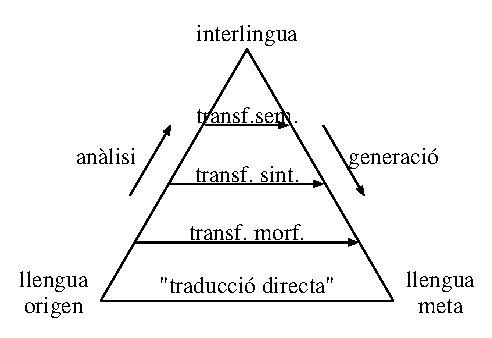
\includegraphics{triangle}
\end{center}
\caption{Com més profunda i complexa és l'anàlisi del text origen, més
  senzilla és (menys esforç comporta) la transferència a la
  representació corresponent de la llengua meta i més complexa la
  generació.  L'anàlisi del text origen és tan profunda en els
  sistemes d'interlingua clàssics que no és necessària la
  transferència.}
\label{fg:triangle}
\end{figure}

Les interlingües poden ser de molts tipus. Els sistemes clàssics usen
representacions estructurals més o menys complexes per a representar
les relacions semàntiques entre els elements de la frase. 
% (de l'estil de les de la solució a l'exercici~\ref{exer:agradar}).  
Però les interlingües no han de ser necessàriament el resultat d'una
anàlisi profunda: el que han de ser necessàriament és \emph{neutrals};
per exemple, alguns sistemes històrics com DLT
\citep[cap.~17]{hutchins92b} usen com a \emph{interlingua} una llengua
\emph{pivot} ``natural'' com l'esperanto, amb anotacions que resolen
algunes ambigüitats típiques.\footnote{Aquesta aproximació pot ser
  particularment útil quan les llengües entre les quals ha de traduir
  el sistema tenen una gran similitud sintàctica i semàntica, com en
  el cas de les llengües romàniques, amb l'excepció, potser, del
  romanés.}

En l'intent de representar els significats de totes les frases de
totes les llengües, les interlingües clàssiques acabarien per ser
``models del món''. Això fa que, actualment, només s'hagen
desenvolupat sistemes d'interlingua clàssics per a àmbits temàtics
molt concrets.

Un dels avantatges més importants dels sistemes d'interlingua respecte
dels sistemes de transferència és la facilitat amb què es pot afegir
una llengua nova a un sistema de traducció automàtica multilingüe.
Imaginem tres llengües que anomenarem $L_1$, $L_2$ i $L_3$. Un sistema
complet de transferència que traduïra entre aquestes tres llengües en
els dos sentits tindria tres mòduls d'anàlisi (que anomenarem $A_1$,
$A_2$ i $A_3$), tres mòduls de generació (que anomenarem $G_1$, $G_2$
i $G_3$) i sis mòduls de transferència (que anomenarem $T_{12}$,
$T_{13}$, $T_{23}$, $T_{31}$, $T_{32}$ i $T_{21}$).\footnote{En
  general, per a $N$ llengües $L_1, L_2, \ldots, L_N$ hi hauria $N$
  mòduls d'anàlisi, $N$ mòduls de generació i $N(N-1)$ mòduls de
  transferència.} Afegir un quart idioma $L_4$ al sistema comporta:
\begin{itemize}
\item Crear un nou mòdul d'anàlisi ($A_4$).
\item Crear un nou mòdul de generació ($G_4$).
\item Construir 6 nous mòduls de transferència ($T_{14}$, $T_{24}$,
  $T_{34}$, $T_{41}$, $T_{42}$ i $T_{43}$). Notem que per a aquesta
  última fase són necessaris diversos experts bilingües en sistemes de
  transferència.\footnote{En el cas general d'afegir una llengua a un
    conjunt de $N$ llengües, calen $2N$ nous mòduls de transferència.}
\end{itemize}
La figura~\ref{fg:afetran} il·lustra el cost d'afegir $L_4$ al sistema
de transferència;
\begin{figure}
\begin{center}
%TexCad Options
%\grade{\off}
%\emlines{\off}
%\beziermacro{\on}
%\reduce{\on}
%\snapping{\off}
%\quality{2.00}
%\graddiff{0.01}
%\snapasp{1}
%\zoom{1.00}
{\scriptsize 
\unitlength 0.80mm
\linethickness{0.4pt}
\begin{picture}(155.00,100.00)
\put(110.00,10.00){\makebox(0,0)[cc]{$L_3$}}
\put(110.00,25.00){\makebox(0,0)[cc]{$RA_3$}}
\put(110.00,85.00){\makebox(0,0)[cc]{$RA_1$}}
\put(110.00,100.00){\makebox(0,0)[cc]{$L_1$}}
\put(80.00,55.00){\makebox(0,0)[cc]{$RA_2$}}
\put(65.00,55.00){\makebox(0,0)[cc]{$L_2$}}
\put(140.00,55.00){\makebox(0,0)[cc]{$RA_4$}}
\put(155.00,55.00){\makebox(0,0)[cc]{$L_4$}}
%\vector(152.00,57.00)(143.00,57.00)
\put(143.00,57.00){\vector(-1,0){0.2}}
\put(152.00,57.00){\line(-1,0){9.00}}
%\end
%\vector(143.00,53.00)(152.00,53.00)
\put(152.00,53.00){\vector(1,0){0.2}}
\put(143.00,53.00){\line(1,0){9.00}}
%\end
%\vector(108.00,97.00)(108.00,88.00)
\put(108.00,88.00){\vector(0,-1){0.2}}
\put(108.00,97.00){\line(0,-1){9.00}}
%\end
%\vector(112.00,88.00)(112.00,97.00)
\put(112.00,97.00){\vector(0,1){0.2}}
\put(112.00,88.00){\line(0,1){9.00}}
%\end
%\vector(68.00,53.00)(77.00,53.00)
\put(77.00,53.00){\vector(1,0){0.2}}
\put(68.00,53.00){\line(1,0){9.00}}
%\end
%\vector(77.00,57.00)(68.00,57.00)
\put(68.00,57.00){\vector(-1,0){0.2}}
\put(77.00,57.00){\line(-1,0){9.00}}
%\end
%\vector(108.00,22.00)(108.00,13.00)
\put(108.00,13.00){\vector(0,-1){0.2}}
\put(108.00,22.00){\line(0,-1){9.00}}
%\end
%\vector(112.00,13.00)(112.00,22.00)
\put(112.00,22.00){\vector(0,1){0.2}}
\put(112.00,13.00){\line(0,1){9.00}}
%\end
\put(104.00,93.00){\makebox(0,0)[cc]{$A_1$}}
\put(116.00,93.00){\makebox(0,0)[cc]{$G_1$}}
\put(72.00,61.00){\makebox(0,0)[cc]{$G_2$}}
\put(72.00,49.00){\makebox(0,0)[cc]{$A_2$}}
\put(148.00,49.00){\makebox(0,0)[cc]{$G_4$}}
\put(148.00,61.00){\makebox(0,0)[cc]{$A_4$}}
\put(116.00,17.00){\makebox(0,0)[cc]{$A_3$}}
\put(104.00,17.00){\makebox(0,0)[cc]{$G_3$}}
\put(108.00,82.00){\vector(0,-1){47.00}}
\put(83.00,53.00){\vector(1,0){47.00}}
\put(137.00,57.00){\vector(-1,0){47.00}}
\put(112.00,28.00){\vector(0,1){47.00}}
\put(137.00,57.00){\vector(-1,1){21.00}}
\put(108.00,81.67){\vector(-1,-1){21.00}}
\put(83.00,53.00){\vector(1,-1){21.00}}
\put(112.00,28.00){\vector(1,1){21.00}}
\put(83.00,53.00){\vector(1,1){21.00}}
\put(112.00,28.00){\vector(-1,1){22.00}}
\put(137.00,57.00){\vector(-1,-1){21.00}}
\put(108.00,82.00){\vector(1,-1){22.00}}
\put(130.00,70.00){\makebox(0,0)[cc]{$T_{41}$}}
\put(125.00,35.00){\makebox(0,0)[cc]{$T_{34}$}}
\put(90.00,40.00){\makebox(0,0)[cc]{$T_{23}$}}
\put(95.00,75.00){\makebox(0,0)[cc]{$T_{12}$}}
\put(100.00,65.00){\makebox(0,0)[cc]{$T_{21}$}}
\put(120.33,45.33){\makebox(0,0)[cc]{$T_{43}$}}
\put(120.00,65.00){\makebox(0,0)[cc]{$T_{14}$}}
\put(100.00,45.00){\makebox(0,0)[cc]{$T_{32}$}}
\put(100.00,50.00){\makebox(0,0)[cc]{$T_{24}$}}
\put(120.00,60.00){\makebox(0,0)[cc]{$T_{42}$}}
\put(116.00,45.33){\makebox(0,0)[cc]{$T_{31}$}}
\put(105.00,65.00){\makebox(0,0)[cc]{$T_{13}$}}
\put(45.00,10.00){\makebox(0,0)[cc]{$L_3$}}
\put(45.00,25.00){\makebox(0,0)[cc]{$RA_3$}}
\put(45.00,85.00){\makebox(0,0)[cc]{$RA_1$}}
\put(45.00,100.00){\makebox(0,0)[cc]{$L_1$}}
\put(15.00,55.00){\makebox(0,0)[cc]{$RA_2$}}
\put(0.00,55.00){\makebox(0,0)[cc]{$L_2$}}
%\vector(43.00,97.00)(43.00,88.00)
\put(43.00,88.00){\vector(0,-1){0.2}}
\put(43.00,97.00){\line(0,-1){9.00}}
%\end
%\vector(47.00,88.00)(47.00,97.00)
\put(47.00,97.00){\vector(0,1){0.2}}
\put(47.00,88.00){\line(0,1){9.00}}
%\end
%\vector(3.00,53.00)(12.00,53.00)
\put(12.00,53.00){\vector(1,0){0.2}}
\put(3.00,53.00){\line(1,0){9.00}}
%\end
%\vector(12.00,57.00)(3.00,57.00)
\put(3.00,57.00){\vector(-1,0){0.2}}
\put(12.00,57.00){\line(-1,0){9.00}}
%\end
%\vector(43.00,22.00)(43.00,13.00)
\put(43.00,13.00){\vector(0,-1){0.2}}
\put(43.00,22.00){\line(0,-1){9.00}}
%\end
%\vector(47.00,13.00)(47.00,22.00)
\put(47.00,22.00){\vector(0,1){0.2}}
\put(47.00,13.00){\line(0,1){9.00}}
%\end
\put(39.00,93.00){\makebox(0,0)[cc]{$A_1$}}
\put(51.00,93.00){\makebox(0,0)[cc]{$G_1$}}
\put(7.00,61.00){\makebox(0,0)[cc]{$G_2$}}
\put(7.00,49.00){\makebox(0,0)[cc]{$A_2$}}
\put(51.00,17.00){\makebox(0,0)[cc]{$A_3$}}
\put(39.00,17.00){\makebox(0,0)[cc]{$G_3$}}
\put(43.00,82.00){\vector(0,-1){47.00}}
\put(47.00,28.00){\vector(0,1){47.00}}
\put(43.00,81.67){\vector(-1,-1){21.00}}
\put(18.00,53.00){\vector(1,-1){21.00}}
\put(18.00,53.00){\vector(1,1){21.00}}
\put(47.00,28.00){\vector(-1,1){22.00}}
\put(25.00,40.00){\makebox(0,0)[cc]{$T_{23}$}}
\put(30.00,75.00){\makebox(0,0)[cc]{$T_{12}$}}
\put(35.00,65.00){\makebox(0,0)[cc]{$T_{21}$}}
\put(35.00,45.00){\makebox(0,0)[cc]{$T_{32}$}}
\put(51.00,45.33){\makebox(0,0)[cc]{$T_{31}$}}
\put(40.00,65.00){\makebox(0,0)[cc]{$T_{13}$}}
\end{picture}
}
\end{center}
\caption{Cost d'afegir una quarta llengua $L_4$ a un sistema de
  transferència. Les entitats $RA_1$ a $RA_4$ són les representacions
  abstractes (tant RALO com RALM) que usen els mòduls de
  transferència.}
\label{fg:afetran}
\end{figure}
En canvi, en un sistema d'interlingua no hi ha mòduls de
transferència; un sistema trilingüe basat en una interlingua tindria
només sis mòduls: tres d'anàlisi ($A'_1$, $A'_2$ i $A'_3$) i tres de
generació ($G'_1$, $G'_2$ i $G'_3$). Queda clar que els mòduls
d'anàlisi i de generació en aquests sistemes són més complexos que en
el cas de transferència (ja que han de fer transformacions cap a
estructures lingüísticament neutrals), però també és clar l'avantatge
del sistema d'interlingua a l'hora d'afegir-hi la llengua $L_4$: només
cal dissenyar dos mòduls nous, $A'_4$ i $G'_4$, i per a dissenyar-los
només necessitem una persona que conega bé la llengua $L_4$ i la
interlingua $I$ que usa el sistema. La figura~\ref{fg:afeinte}
il·lustra el cost d'afegir $L_4$ al sistema.
\begin{figure}
\begin{center}
%TexCad Options
%\grade{\off}
%\emlines{\off}
%\beziermacro{\on}
%\reduce{\on}
%\snapping{\off}
%\quality{2.00}
%\graddiff{0.01}
%\snapasp{1}
%\zoom{1.00}
\unitlength 1.00mm
\linethickness{0.4pt}
\begin{picture}(100.00,50.00)
\put(60.00,30.00){\makebox(0,0)[cc]{$L_2$}}
\put(80.00,10.00){\makebox(0,0)[cc]{$L_3$}}
\put(80.00,50.00){\makebox(0,0)[cc]{$L_1$}}
\put(100.00,30.00){\makebox(0,0)[cc]{$L_4$}}
\put(80.00,30.00){\makebox(0,0)[cc]{$I$}}
%\vector(78.00,33.00)(78.00,45.00)
\put(78.00,45.00){\vector(0,1){0.2}}
\put(78.00,33.00){\line(0,1){12.00}}
%\end
%\vector(82.00,47.00)(82.00,35.00)
\put(82.00,35.00){\vector(0,-1){0.2}}
\put(82.00,47.00){\line(0,-1){12.00}}
%\end
%\vector(83.00,32.00)(95.00,32.00)
\put(95.00,32.00){\vector(1,0){0.2}}
\put(83.00,32.00){\line(1,0){12.00}}
%\end
%\vector(97.00,28.00)(85.00,28.00)
\put(85.00,28.00){\vector(-1,0){0.2}}
\put(97.00,28.00){\line(-1,0){12.00}}
%\end
%\vector(82.00,27.00)(82.00,15.00)
\put(82.00,15.00){\vector(0,-1){0.2}}
\put(82.00,27.00){\line(0,-1){12.00}}
%\end
%\vector(78.00,13.00)(78.00,25.00)
\put(78.00,25.00){\vector(0,1){0.2}}
\put(78.00,13.00){\line(0,1){12.00}}
%\end
%\vector(77.00,28.00)(65.00,28.00)
\put(65.00,28.00){\vector(-1,0){0.2}}
\put(77.00,28.00){\line(-1,0){12.00}}
%\end
%\vector(63.00,32.00)(75.00,32.00)
\put(75.00,32.00){\vector(1,0){0.2}}
\put(63.00,32.00){\line(1,0){12.00}}
%\end
\put(70.00,36.00){\makebox(0,0)[cc]{$A'_2$}}
\put(90.00,36.00){\makebox(0,0)[cc]{$G'_4$}}
\put(90.00,24.00){\makebox(0,0)[cc]{$A'_4$}}
\put(70.00,24.00){\makebox(0,0)[cc]{$G'_2$}}
\put(74.00,40.00){\makebox(0,0)[cc]{$G'_1$}}
\put(74.00,20.00){\makebox(0,0)[cc]{$A'_3$}}
\put(86.00,20.00){\makebox(0,0)[cc]{$G'_3$}}
\put(86.00,40.00){\makebox(0,0)[cc]{$A'_1$}}
\put(10.00,30.00){\makebox(0,0)[cc]{$L_2$}}
\put(30.00,10.00){\makebox(0,0)[cc]{$L_3$}}
\put(30.00,50.00){\makebox(0,0)[cc]{$L_1$}}
\put(30.00,30.00){\makebox(0,0)[cc]{$I$}}
%\vector(28.00,33.00)(28.00,45.00)
\put(28.00,45.00){\vector(0,1){0.2}}
\put(28.00,33.00){\line(0,1){12.00}}
%\end
%\vector(32.00,47.00)(32.00,35.00)
\put(32.00,35.00){\vector(0,-1){0.2}}
\put(32.00,47.00){\line(0,-1){12.00}}
%\end
%\vector(32.00,27.00)(32.00,15.00)
\put(32.00,15.00){\vector(0,-1){0.2}}
\put(32.00,27.00){\line(0,-1){12.00}}
%\end
%\vector(28.00,13.00)(28.00,25.00)
\put(28.00,25.00){\vector(0,1){0.2}}
\put(28.00,13.00){\line(0,1){12.00}}
%\end
%\vector(27.00,28.00)(15.00,28.00)
\put(15.00,28.00){\vector(-1,0){0.2}}
\put(27.00,28.00){\line(-1,0){12.00}}
%\end
%\vector(13.00,32.00)(25.00,32.00)
\put(25.00,32.00){\vector(1,0){0.2}}
\put(13.00,32.00){\line(1,0){12.00}}
%\end
\put(20.00,36.00){\makebox(0,0)[cc]{$A'_2$}}
\put(20.00,24.00){\makebox(0,0)[cc]{$G'_2$}}
\put(24.00,40.00){\makebox(0,0)[cc]{$G'_1$}}
\put(24.00,20.00){\makebox(0,0)[cc]{$A'_3$}}
\put(36.00,20.00){\makebox(0,0)[cc]{$G'_3$}}
\put(36.00,40.00){\makebox(0,0)[cc]{$A'_1$}}
\end{picture}
\end{center}
\caption{Cost d'afegir una quarta llengua $L_4$ a un sistema
  d'interlingua.}
\label{fg:afeinte}
\end{figure} 

\section{Sistemes de traducció automàtica basats en corpus}
\label{ss:induc}
Totes les tècniques de traducció automàtica descrites fins ara són de
naturalesa \emph{deductiva}, és a dir, estan basades en teories i
coneixements lingüístics sobre la traducció. Però recentment (sobretot
en els primers anys del tercer mil·lenni) s'està produint un
creixement espectacular de tècniques \emph{inductives} de traducció
automàtica, en les quals el sistema \emph{aprén} automàticament a
traduir entre dues llengües a partir d'un corpus paral·lel
suficientment gran d'oracions en LO acompanyades de la seua traducció
a la LM (vegeu l'apartat~\ref{ss:bitextos}). Aquestes aproximacions
inductives també reben el nom de \emph{traducció automàtica basada en
  corpus}.

\subsection{Sistemes de traducció automàtica estadística}
\label{ss:tae}
La principal tècnica de traducció automàtica basada en corpus es la
\emph{traducció automàtica estadística} (en anglés \emph{statistical
  machine translation}; SMT), la qual va ser inventada cap a finals
dels huitanta per un grup d'investigadors d'IBM \citep{brown90j}; els
sistemes actuals són una evolució d'aquests.

A l'hora de traduir hi ha una diferència fonamental entre els sistemes
basats en regles o coneixement i els sistemes estadístics: mentres que
els sistemes basat en regles produeixen únicament una traducció, els
sistemes estadístics generen una gran quantitat d'\emph{hipòtesis de
  traducció} (idealment totes les possibles) i utilitzen models
estadístics per \emph{puntuar} les hipòtesis generades i escollir la
millor de totes. Els principals models estadístics que s'usen per
puntuar les hipòtesis de traducció són el \emph{model de traducció} i
el \emph{model de llengua}, els quals s'expliquen més avall. La
combinació d'aquests models fa que la hipòtesi de traducció que rep
la puntuació \emph{global} més alta no siga necessàriament la hipòtesi
de traducció millor segons cada model per separat.

\begin{figure}
\centering
\begin{tabular}{p{6cm}|p{6cm}}
  \multicolumn{1}{c|}{\textbf{Anglés}} & \multicolumn{1}{c}{\textbf{Espanyol}}\\
  \hline
  It has been exciting in many ways . &
  Ha sido un trabajo apasionante en varios sentidos . \\
  \hline
  As the shadow rapporteurs know , this has been my first report
  during my time in Parliament and it has been a good learning
  experience . &
  Como bien saben los ponentes alternativos , éste ha sido el primer
  informe en el que he trabajado durante mi mandato parlamentario , y
  me ha venido muy bien como experiencia formativa . \\
  \hline
  It has also been very challenging to work on three reports and
  therefore also with other rapporteurs . &
  También ha sido un gran desafío trabajar en tres informes , y por lo
  tanto con otros ponentes . \\
  \hline
  It has been exciting . &
  Ha sido emocionante . \\
  \hline
\end{tabular}
\caption{Oracions paral·leles anglés-espanyol extretes del corpus
  paral·lel Europarl (\texttt{http://www.statmt.org/europarl/}) amb
  les actes del Parlament Europeu de període 1996--2011.}
\label{fg:alinora}
\end{figure}


\begin{figure}
\centering
\includegraphics[scale=0.5]{alin-paraules}
\caption{Alineament entre les paraules de l'oració en anglés
  \emph{The white bird decided to fly.} and les paraules de l'oració en
català \emph{El pardal blanc va decidir volar.}}
\label{fg:alinpar}
\end{figure}

El \textbf{model de traducció} s'aprén a partir d'un corpus paral·lel
amb les oracions ja alineades com el que es mostra en la figura
\ref{fg:alinora}. Primerament, s'han d'obtenir els \emph{alineaments
  entre els mots} (vegeu-ne un exemple en la figura \ref{fg:alinpar})
per a després estimar el model de traducció a partir d'aquests
alineaments.

\begin{figure}[tb]
  \centering %
  \subfigure[\label{fg:pasosalin1}Inicialització: Tots els alineament
  són igualment probables.]{\includegraphics[scale=0.5]{ibm1/ibm2}} 

  \subfigure[\label{fg:pasosalin2}Primera iteració: El alineament
  entre \emph{yn} i \emph{gur} guanya
  força.]{\includegraphics[scale=0.5]{ibm1/ibm3}}

  \subfigure[\label{fg:pasosalin3}Segona iteració: El alineament entre
  \emph{pifo} i \emph{ubhfo} guanya
  força.]{\includegraphics[scale=0.5]{ibm1/ibm4}}

  \subfigure[\label{fg:pasosalin4}Tercera i última iteració:
  L'estructura d'alineament que estava ``oculta'' queda al
  descobert.]{\includegraphics[scale=0.5]{ibm1/ibm5}}
  \caption{Exemple que il·lustra el procés iteratiu que permet obtenir
    l'alineament entre les paraules de les oracions d'un corpus
    paral·lel. En aquest exemple el corpus consta de tres oracions
    paral·leles en dos llengües inventades. Aquestes oracions
    paral·leles són: \emph{yn pifo}--\emph{gur ubhfo}, \emph{yn pifo
      oynapi}--\emph{gur juvga ubhfo} i \emph{yn sybe}--\emph{gur
      subjre}. El gruix de les línies que connecten les paraules
    representa la probabilitat de l'alineament.}
\label{fg:pasosalin}
\end{figure}

Tot i que sembla una tasca difícil per a un ordinador, els alineaments
entre els mots es poden obtenir automàticament sense usar cap
coneixement sobre les llengües dels textos a alinear mitjançat un
procés iteratiu. La figura \ref{fg:pasosalin} il·lustra aquest procés
amb un corpus menut de tres oracions paral·leles; si us fixeu, sense
tenir cap coneixement de les llengües (perquè han estat inventades)
les persones també som capaces d'obtenir aquests alineaments. El
procés comença assumint que, per a cada oració paral·lela, tots els
mots de l'oració en LM poden ser traducció de cadascun dels mots de
l'oració en LO, i per tant, els assigna la mateixa probabilitat.  En
cada iteració el programa alineador visita totes les oracions
paral·leles del corpus i va refinant aquestes probabilitats fins que
l'estructura d'alineament queda definida. Aquest refinament es
produeix perquè en cada iteració les probabilitats de la iteració
anterior s'usen per acumular evidència en tot el corpus sobre la
probabilitat de les correspondències entre mots i, a més, perquè els
mots que són traducció mútua solen aparéixer junts en les mateixes
oracions paral·leles, la qual cosa no succeeix si dos mots no són
traducció un de l'altre.

Una vegada obtinguts els alineaments entre els mots, podem aprendre
models probabilístics que indiquen, per exemple, la probabilitat que
la traducció d'un determinat mot en una llengua siga la traducció d'un
determinat mot en l'altra (un model de traducció de paraules o
diccionari bilingüe probabilístic), o la probabilitat que la traducció
d'una seqüència (segment) de mots en una llengua siga la traducció
d'una seqüència (segment) de mots en l'altra (un model de traducció de
segments). Aquest últim model l'usen els sistemes de traducció
automàtica estadística basats en segments bilingües (en anglés
\emph{phrase-based statistical machine translation}; \cite{koehnbook}),
els quals són els més usats en l'actualitat.

Però per produir bones traduccions no podem usar el model de traducció
únicament perquè les traduccions serien poc naturals, gramaticals i
fluides. El motiu és que el model de traducció no té en compte l'ordre
en què apareixen els segments traduïts en la LM, ni el context en què
apareixen els segments en LO a l'hora de puntuar les seues possibles
traduccions. Aquestes deficiències es mitiguen parcialment amb l'ús
d'un model de la LM.

Un \textbf{model de llengua} és un model probabilístic que serveix per
a mesurar la versemblança d'una oració o text en LM; és a dir, la seua
fluïdesa o gramaticalitat.\footnote{S'assumeix que el model de llengua
  s'aprén de textos naturals i gramaticalment correctes en LM.}
Aquests models s'aprenen de forma automàtica a partir d'un corpus de
text en LM i es basen en comptar la freqüència de segments de longitud
fixa, normalment segments de fins a cinc paraules, per evitar assignar
una versemblança nul·la a oracions que, tot i que són correctes, no
apareixen en els corpus d'entrenament.\footnote{Per evitar assignar
  versemblances nul·les a una oració, a més d'utilitzar segments de
  poques paraules, aquests models també usen tècniques de suavitzat
  (en anglés \emph{smoothing}) de les probabilitat.} El model de
llengua té en compte l'ordre de les paraules i per tant assigna una
versemblança major a l'oració \emph{M'agrada menjar pernil del bo} que
a l'oració \emph{del bo menjar pernil M'agrada}, tot i que contenen
els mateixos segments de text (\emph{del bo}, \emph{menjar pernil} i
\emph{M'agrada}). A més té en compte, tot i que indirectament, el
context en què apareixen les paraules en LM, de manera que assigna
una versemblança major a l'oració en espanyol (LM) \emph{No piensa con
  la cabeza} que a l'oració \emph{No piensa con el cabo}, on els
segments \emph{la cabeza} i \emph{el cabo} són dues possibles
traduccions del segment en català \emph{el cap} que apareix en
l'oració en LO \emph{No pensa amb el cap}.

\begin{persabermes}{sistemes de traducció automàtica estadística}
  A més dels models de traducció i de la LM els sistemes de traducció
  automàtica estadística basats en segments bilingües combinen altres
  models per a establir la puntuació global d'una hipòtesi de
  traducció. A continuació es descriuen molt breument aquests models i
  per a què s'usen:
  \begin{description}
  \item[Model de reordenament lèxic:] La seua funció és modelar
    diferents operacions de reordenament que es poden fer a l'hora de
    disposar les traduccions dels segments en LO. Les probabilitats
    d'aquestes operacions depenen dels segments concrets que s'estan
    reordenant i són tres: traducció monòtona (quan no hi ha
    reordenament), reordenament (quan la posició de la traducció del
    segment en qüestió i la de l'anterior s'intercanvien) i traducció
    discontinua (qual la traducció del segment es mou a una altra
    posició en l'oració en LM; es a dir, quan no és cap de les altres
    dues operacions).
  \item[Ponderació lèxica:] Els segments usats per traduir poden ser
    molt llargs (normalment fins a 7 paraules), la qual cosa fa molt
    difícil estimar bé la seua probabilitat de traducció perquè els
    segments llargs solen aparéixer poques vegades en els corpus
    d'entrenament; això fa necessari l'ús d'un altre model per estimar
    la qualitat dels segments bilingües. Aquest model usa les
    probabilitats de traducció entre els mots (un diccionari bilingüe
    probabilístic) per obtenir un indicador de la qualitat d'els
    segments bilingües. Per exemple, la qualitat del segment bilingüe
    (\emph{la comissió de balanços de finançament}, \emph{the funding
      balance comission}), on l'alineament entre els mots és
    \emph{la}--\emph{the}, \emph{comissió}--\emph{comission},
    \emph{balanços}--\emph{balance} i
    \emph{finançament}--\emph{funding}, depén de les probabilitats de
    traducció dels mots que han estat alineats.
  \item[Nombre total de paraules de l'oració:] Quan es puntuen les
    hipòtesis de traducció es multipliquen moltes probabilitats, és a
    dir valors entre 0 i 1, de manera que com més llarga siga una
    traducció més probabilitats es multipliquen i més fàcil és arribar
    a tenir una puntuació molt prop de zero. Això fa que els sistemes
    preferisquen les traduccions curtes. Per a evitar això
    s'introdueix un model que compta el nombre de paraules en la
    hipòtesi de traducció i que fa que tinga relació amb el nombre de
    paraules de l'oració origen.
  \item[Nombre de segments:] Aquest model és similar a l'anterior, però
    comptant el nombre de segments bilingües que s'han usat per a
    produir una hipòtesi de traducció. Com més llargs siguen els
    segments, menys segments s'usaran i més context tindran; i a
    l'inrevés, com més curts siguen els segments més segments faran
    falta per produir la hipòtesi de traducció.
  \end{description}

  Tots aquests models (i els anteriors) es combinen per a obtenir una
  puntuació global per a cada hipòtesi de traducció i poder escollir
  així la millor. Aquesta combinació es fa assignant un pes
  (importància) a cada model que s'obté mitjançat un procés automàtic
  (\emph{tuning}) que intenta maximitzar la \emph{qualitat} de les
  traduccions proporcionades pel sistema en traduir un corpus de
  \emph{desenvolupament}.  

  Consulteu el llibre de \citet{koehnbook} per saber més sobre els
  models que s'usen per a traduir, el procés de \emph{tuning} i les
  mesures automàtiques de la qualitat que usen.
\end{persabermes}


\begin{persabermes}{sistemes basats en corpus}
  Hi ha hagut altres aproximacions inductives a la traducció
  automàtica, com ara els sistemes de \emph{traducció automàtica
    basada en exemples}, tot i que a hores d'ara ja no s'usen.  La
  \emph{traducció automàtica basada en exemples} intenta construir
  \emph{plantilles} de traducció a partir dels exemples observats en
  el corpus d'oracions paral·leles i \emph{generalitzar-les} perquè
  servisquen en noves situacions. Per exemple, si sabem que el
  substantiu anglés \emph{ski} es tradueix per \emph{esquí} i que la
  locució substantiva \emph{ski station} es tradueix per \emph{estació
    d'esquí} podem generalitzar aquesta última locució substituint
  \emph{ski} per qualsevol altres substantiu $N$, de manera que la
  traducció de ``$N$ \emph{station}'' és ``estació de $N$''; així, si
  la traducció de \emph{train} és \emph{tren}, la traducció de
  \emph{train station} és \emph{estació de tren}, etc. (exemple pres
  de \citealt{carl01j}). Fixeu-vos que la traducció automàtica basada
  en exemples pot necessitar que la mostra de frases i traduccions
  estiga, a més, anotada lingüísticament (en l'exemple, indicant quins
  mots o estructures funcionen com un nom).
\end{persabermes}


\section{Qüestions i exercicis}
Els exercicis marcats amb (*) són més difícils.

\begin{enumerate}
\item Els sistemes de traducció mot per mot poden cometre, per
  exemple, errors en la concordança de gènere o de nombre.  Elegiu
  dues llengües $L_1$ i $L_2$ i poseu almenys dos exemples de
  traduccions mot per mot de $L_1$ a $L_2$ amb problemes de
  concordança.

\item (*) \label{ex:cascat} CasCat és un sistema de traducció
  automàtica de l'espanyol al català que usa regles que reordenen
  seqüències de formes lèxiques segons les categories lèxiques. Les
  regles s'apliquen de la manera usual: d'esquerra a dreta, reordenant
  la seqüència més llarga possible, i sense que se solapen les àrees
  reordenades.  Heus ací algunes frases espanyoles amb {\em cuyo}, les
  traduccions produïdes per CasCat, i, on la traducció és incorrecta,
  una alternativa acceptable.
  \begin{enumerate}
  \item \emph{La chica cuyos compañeros murieron es china} \newline
    {\em La noia els companys de la qual van morir és xinesa}
  \item \emph{La chica cuyos compañeros de clase murieron es china}
    \newline \emph{La noia els companys de classe de la qual van morir
      és xinesa}
  \item \emph{La chica cuyos compañeros mayores murieron es china}
    \newline \emph{La noia els companys grans de la qual van morir és
      xinesa}
  \item \emph{La chica cuyos compañeros de clase de francés murieron
      es china} \newline \emph{*La noia els companys de classe de la
      qual de francès van morir és xinesa} \newline (\emph{La noia els
      companys de classe de francès de la qual van morir és xinesa})
  \item \emph{La chica cuyos compañeros mayores de classe murieron es
      china} \newline \emph{*La noia els companys grans de la qual de
      classe van morir és xinesa} \newline (\emph{La noia els companys
      grans de classe de la qual van morir és xinesa})
  \item \emph{La chica cuyos compañeros mayores de clase de francés
      murieron es china} \newline \emph{*La noia els companys grans de
      la qual de classe de francès van morir és xinesa} \newline
    (\emph{La noia els companys grans de classe de francès de la qual
      van morir és xinesa})
  \end{enumerate}
  Les traduccions inacceptables estan marcades amb un asterisc.
  Proposeu un conjunt de regles de reordenament que expliquen el
  conjunt de traduccions observat. En quins casos es ``trenquen''
  sintagmes?

\item La multinacional WorldTrans ha decidit ampliar el seu sistema de
  traducció automàtica multilingüe LetTrans (que tradueix
  correspondència comercial entre qualssevol dues llengües d'un grup
  de quinze) i afegir-hi la capacitat de traduir del suahili a les
  quinze llengües i de les quinze llengües cap al suahili. En una
  oferta de treball, WorldTrans demana experts en suahili però no
  demana cap expert en traducció entre suahili i cap de les quinze
  llengües. Quina classe de sistema de traducció automàtica és
  LetTrans?  Justifiqueu la resposta.

\item (*) Imagineu que teniu un sistema de traducció automàtica que
  treballa amb dues llengües, diguem-ne $A$ i $B$, en els dos sentits
  de traducció: $A{\rightarrow}B$ i $B{\rightarrow}A$, que traduïm un
  text origen $T$ en llengua $A$ a la llengua $B$ mitjançant aquest
  traductor automàtic, generant un text $T'$, i que després usem
  aquest mateix sistema per a traduir $T'$ de nou a la llengua $A$;
  anomenarem $T''$ el nou text en llengua $A$.
  \begin{equation}
    T \stackrel{\scriptsize A\rightarrow
      B}{\longrightarrow}T'\stackrel{\scriptsize B\rightarrow
      A}{\longrightarrow} T''
  \end{equation}
  El text $T''$ serà previsiblement diferent del text $T$.  Trieu dues
  llengües $A$ i $B$ i indiqueu quins canvis són previsibles,
  classificant-los segons la naturalesa lingüística dels fenòmens que
  han causat els canvis, explicant la raó del resultat si cal amb un
  exemple. Heu d'indicar \emph{tres tipus diferents} de canvi.

\item (*) Imagineu que sou part d'un equip de desenvolupament d'un
  sistema de traducció automàtica de l'anglés al català basat en
  l'estratègia de transferència morfològica avançada
  (apartat~\ref{s3:STMorf}). Els informàtics del projecte us demanen
  consell sobre les regles de reordenament del sistema, ja que, per
  motius tècnics, només poden afegir-n'hi tres.
      
  Indiqueu quines serien les 3 regles que proposaríeu, tenint en
  compte que han de produir, com a mínim, tres oracions ben traduïdes
  en el corpus d'oracions següents (la traducció ideal s'indica entre
  parèntesis, tot i que no sempre podrà ser aconseguida):
  \begin{enumerate}
  \item \emph{A dark autumn night} (\emph{Una nit fosca de
      tardor})
  \item \emph{A high tide} (\emph{Una marea alta}) 
  \item \emph{A magic dark silhouette} (\emph{Una silueta fosca
      màgica})
  \item \emph{An autumn tide} (\emph{Una marea de tardor})
  \item \emph{A dark magic silhouette} (\emph{Una silueta màgica
      fosca})
  \item \emph{A dark autumn high tide} (\emph{Una marea alta de
      tardor fosca})
  \item \emph{A dark night} (\emph{Una nit fosca})
  \end{enumerate}
    
  Deixeu de banda la concordança i centreu-vos només en els
  reordenaments. Assenyaleu quina seria la traducció del sistema per a
  totes les oracions anteriors usant el conjunt de regles que heu
  proposat.

\item Quina és l'operació inversa de l'anàlisi morfològica?
  \begin{enumerate}
  \item L'obtenció de la forma lèxica d'un mot a partir de la forma
    superficial.
  \item La generació morfològica.
  \item La transferència morfològica.
  \end{enumerate}

\item La traducció automàtica per transferència és sempre...
  \begin{enumerate}
  \item ... morfològica.
  \item ... directa.
  \item ... indirecta.
  \end{enumerate}

\item (*) Dues traduccions possibles del mot català \emph{cap} a
  l'espanyol són \emph{cabe} o \emph{cabeza}. Com podria fer l'elecció
  adequada un sistema de traducció automàtica?
  \begin{enumerate}
  \item Posant-hi la traducció més probable, basada en les freqüències
    d'ús dels mots.
  \item Usant informació morfosintàctica, ja que en la posició
    concreta de la frase podria anar només un verb o un substantiu.
  \item No podria, perquè les dues traduccions són sempre possibles en
    qualsevol frase.
  \end{enumerate}

\item Quines de les següents representacions intermèdies son més
  costoses d'obtenir a partir de les frases?
  \begin{enumerate}
  \item Els arbres d'anàlisi sintàctica corresponents.
  \item Les seqüències de categories morfològiques corresponents.
  \item Les estructures semàntiques superficials corresponents.
  \end{enumerate}

%\item Només una d'aquestes operacions és esperable en una situació
%  normal de traducció automàtica. Quina?
%  \begin{enumerate}
%  \item La postedició en un sistema de traducció automàtica usat per a
%    l'assimilació.
%  \item Una fase complexa de transferència en un sistema
%    d'interlingua.
%  \item La preedició en un sistema de traducció automàtica usat per a
%    la disseminació.
%  \end{enumerate}
      
\item L'anàlisi morfològica pren una oració i...
  \begin{enumerate}
  \item ... produeix un arbre d'anàlisi.
  \item ... produeix, per a cada mot, totes les formes superficials
    corresponents.
  \item ... produeix, per a cada mot, totes les tripletes
    lema--categoria--informació morfològica possibles.
  \end{enumerate}

\item Quines són les fases bàsiques d'un sistema de traducció
  automàtica indirecta?
  \begin{enumerate}
  \item Anàlisi, generació i traducció.
  \item Anàlisi, transferència i generació.
  \item Anàlisi i transferència.
  \end{enumerate}

\item Quin dels següents tipus de sistema de traducció automàtica
  faciliten més l'addició d'una nova llengua?
  \begin{enumerate}
  \item Els sistemes de transferència morfològica avançada.
  \item Els sistemes de transferència semàntica superficial.
  \item Els sistemes d'\emph{interlingua}.
  \end{enumerate}

\item Quin dels següents tipus de sistema de traducció automàtica
  tenen la fase de transferència més senzilla possible?
  \begin{enumerate}
  \item Els sistemes de transferència morfològica avançada.
  \item Els sistemes de transferència semàntica superficial.
  \item Els sistemes d'\emph{interlingua}.
  \end{enumerate}

\item Primerament, elegiu un idioma meta (francés, anglés o alemany) i
  un idioma origen (català o espanyol). Després, per als idiomes
  elegits, doneu un exemple de traducció mot a mot inacceptable en
  \emph{tres} d'aquests cinc casos:
  \begin{enumerate}
  \item homografia mal resolta d'un mot
  \item polisèmia mal resolta d'un mot
  \item problemes de concordança
  \item ambigüitat estructural mal resolta
  \item problemes amb l'ordre dels mots
  \end{enumerate}
      
\item \emph{Interlingua}, a més de ser el nom de la representació
  intermèdia dels sistemes indirectes sense transferència, és el d'una
  llengua artificial bàsicament d'arrel llatina, amb una flexió
  simplificada, i amb un vocabulari dissenyat per a ser comprensible a
  molts europeus.  Una característica important d'interlingua és que
  els determinants (\emph{un}, \emph{le}, \emph{alcun}, \emph{iste},
  \emph{mi}, \emph{tu}, etc.) i els adjectius són invariables. Els
  plurals dels noms es fan amb \emph{-s} o \emph{-es}.  Imagineu que
  tenim un sistema de transferència morfològica avançada que tradueix
  d'interlingua al català (o a l'espanyol) usant aquestes quatre
  regles:
  \begin{itemize}
  \item[$R_1$] detecta \textbf{det}--\textbf{n} i escriu
    \textsf{trad}(\textbf{det})--\textsf{trad}(\textbf{n}), fent
    concordar \textsf{trad}(\textbf{det}) en gènere i en nombre amb
    \textsf{trad}(\textbf{n})
  \item[$R_2$] detecta \textbf{det}--\textbf{n}--\textbf{adj} i escriu
    \textsf{trad}(\textbf{det})--\textsf{trad}(\textbf{n})-\textsf{trad}(\textbf{adj}),
    fent concordar \textsf{trad}(\textbf{det}) i
    \textsf{trad}(\textbf{adj})en gènere i en nombre amb
    \textsf{trad}(\textbf{n})
  \item[$R_3$] detecta \textbf{n}--\textbf{adj} i escriu
    \textsf{trad}(\textbf{n})--\textsf{trad}(\textbf{adj}), fent
    concordar \textsf{trad}(\textbf{adj}) en gènere i en nombre amb
    \textsf{trad}(\textbf{n})
  \item[$R_4$] detecta \textbf{adj}--\textbf{n} i escriu
    \textsf{trad}(\textbf{n})--\textsf{trad}(\textbf{adj}), fent
    concordar \textsf{trad}(\textbf{adj}) en gènere i en nombre amb
    \textsf{trad}(\textbf{n})
  \end{itemize}
  Si no es pot usar informació de concordança, la traducció dels
  determinants i els adjectius es fa en masculí singular.  Indica
  quines traduccions al català (o a l'espanyol) produirà aquest
  sistema per a les frases següents i per què:
  \begin{enumerate}
  \item \emph{Un longe viage}
  \item \emph{Un longe viages}
  \item \emph{Un viages longe}
  \item \emph{Longe viages}
  \item \emph{Un governamento non democratic}
  \item \emph{Un governamentos non democratic}
  \item \emph{Tu melior ideales}
  \item \emph{Un bon solution}
  \end{enumerate}

\item (*) La traducció d'una oració es pot veure com una interpretació
  d'aquesta (és a dir, com l'expressió en la llengua meta del seu
  significat). El \emph{principi de composicionalitat semàntica}
  postula que la interpretació d'una oració es construeix combinant
  les interpretacions dels mots seguint precisament les agrupacions
  successives (constituents) que indica l'arbre d'anàlisi sintàctica
  de l'oració, partint dels mots i anant cap a l'arrel de
  l'arbre. Indiqueu en quin (o quins) tipus de sistema de traducció
  automàtica trobem un disseny que aplica, exactament o
  aproximadament, el principi de composicionalitat. Raoneu breument la
  resposta.
      
\item \label{ex:zkanagg} El programari que porten instal·lat les naus
  de la confederació galàctica inclou un programa que tradueix una de
  les llengües majoritàries del planeta Zkanagg, el tazkannwat, al
  català. El sistema és un sistema de transferència morfològica
  avançada estàndard, que llegeix els textos d'esquerra a dreta, mot a
  mot, busca en l'entrada els patrons de categories lèxiques que conté
  en el seu catàleg, selecciona el més llarg, reordena i concorda els
  mots del patró, els escriu, i continua després de la zona
  reordenada. Algunes traduccions són errònies perquè el sistema no té
  un catàleg massa complet de regles. Fixeu-vos en els exemples i
  digueu quins són els patrons que detecta i quines les regles de
  reordenament associades.
     \begin{example}
     \gll Thlong u knaar uw phlagyw.
          {Va adquirir} el navegant el-OBJ control-OBJ
     \glt TA: El navegant va adquirir el control (correcta).
     \glend
     \end{example}
     \begin{example}
     \gll Thlong u knaar qimratt uw phlagyw.
          {Va adquirir} el navegant estelar el-OBJ control-OBJ
     \glt TA: El navegant estelar va adquirir el control (correcta).
     \glend
     \end{example}
     \begin{example}
     \gll Thlong u knaar na Zkannag uw phlagyw.
          {Va adquirir} el navegant de Zkannag el-OBJ control-OBJ
     \glt TA: El navegant de Zkannag va adquirir el control (correcta).
     \glend
     \end{example}
     \begin{example}
     \gll Thlong u knaar qimratt na Zkannag uw phlagyw.
          {Va adquirir} el navegant estelar de Zkannag el-OBJ control-OBJ
     \glt TA: *El navegant estelar va adquirir de Zkannag el control.
     \glt Correcta: El navegant estelar de Zkannag va adquirir el control.
     \glend
     \end{example}

% \item \label{exer:agradar} Les estructures sintàctiques usades per diverses llengües a
%   l'hora d'expressar el fet que alguna acció agrada a algú són molt
%   diverses. La frase ``m'agrada nadar'' té una estructura sintàctica molt
%   diferent en anglés (\ref{ex:angles}) i en alemany (\ref{ex:alemany}).
% \begin{example}
% \gll Peter likes swimming.
%      Peter s'estima nadant.
% \glt\glend
% \label{ex:angles}
% \end{example}
% \begin{example}
% \gll Peter schwimmt gern.
%      Peter nada {amb gust}.
% \glt\glend
% \label{ex:alemany}
% \end{example}
% Altre exemple el tenim en la frase  ``li diuen Joan'':
% \begin{example}
% \gll He is called Joan.
%      Ell és anomenat Joan.
% \glt\glend
% \label{ex:angles2}
% \end{example}
% \begin{example}
% \gll Er hei{\ss}t Joan.
%      Ell {s'anomena}  Joan.
% \glt\glend
% \label{ex:alemany2}
% \end{example}
% En canvi, les estructures que serveixen per a expressar altres
% conceptes poden ser completament paral·leles. Quines conseqüències té
% això per al disseny d'un sistema de traducció automàtica de
% transferència sintàctica entre llengües amb aquestes característiques?
% Com es podrien evitar els problemes observats?

\item Els mots no són tots igualment freqüents en els textos. De fet,
  si ordenem els mots d'un gran corpus de text real (de qualsevol
  tipus i de qualsevol idioma) pel nombre de vegades que hi apareixen,
  començant pel més freqüent, el nombre d'aparicions es redueix
  dramàticament segons que anem baixant per la llista. Típicament, el
  mot més freqüent pot arribar a constituir el 10\% de tot el text,
  però el segon només cobreix al voltant del 5\%, el tercer al voltant
  del 3\%, etc.; quan arribem al 100é mot més freqüent ja hem de
  parlar del 0,1\% (una vegada cada 1.000 mots), i si arribem a la
  posició 1000, del 0,01\% (una vegada cada 10.000 mots).  En resum,
  la distribució no és gens homogènia: uns pocs mots són els més
  freqüents i la majoria són moltíssim menys freqüents. De fet, és
  típic que la majoria dels mots siguen \emph{hapax legomena}, és a
  dir, mots que han aparegut només una vegada en tot el corpus. Si
  haguéreu de supervisar la construcció dels diccionaris d'un sistema
  de traducció automàtica, per a què us podrien servir aquestes
  constatacions estadístiques?

\item (*) \label{ex:postres} Els sistemes de traducció automàtica
  entre dues llengües amb sintaxi similar no necessiten fer massa
  reordenaments perquè l'ordre dels mots no varia massa d'una llengua
  a altra. A pesar d'això, la traducció mot per mot no és practicable
  perquè el gènere i el nombre gramatical d'alguns substantius varia i
  els adjectius, articles, etc., que l'acompanyen no concordarien
  correctament: cast. {\em una señal muy clara\/} $\rightarrow$
  cat. *{\em una senyal molt clara} (correcte: {\em un senyal molt
    clar\/}); cast. {\em me gusta la leche fría} $\rightarrow$
  ital. *{\em mi piace la latte fredda\/} (correcte: {\em mi piace il
    latte freddo}). Una manera d'identificar zones on s'ha d'establir
  la concordança és detectar seqüències de mots, de manera similar a
  com es fa en els sistemes de transferència morfològica, però sense
  reordenar-les. Per exemple, detectar la seqüència {\bf art}--{\bf
    subst} pot servir per propagar el gènere i el nombre del
  substantiu a l'article. Fixeu-vos en les frases espanyoles següents
  i les traduccions al català fetes per un sistema que usa aquesta
  estratègia i deduïu quines són les seqüències que detecta i quines
  no. Justifiqueu la vostra resposta.
  \begin{enumerate}
  \item \emph{Nos ofreció un postre} $\rightarrow$ \emph{Ens va oferir
      unes postres\/}
  \item \emph{Nos ofreció un postre buenísimo} $\rightarrow$ \emph{Ens
      va oferir unes postres boníssimes\/}
  \item \emph{Nos ofreció un buen postre} $\rightarrow$ \emph{*Ens va
      oferir un bon postres\/}
  \item \emph{Nos ofreció un postre típico buenísimo\/} $\rightarrow$
    \emph{*Ens va oferir unes postres típiques boníssim\/}
  \item \emph{Nos ofreció un postre muy bueno} $\rightarrow$ \emph{*Ens
      va oferir unes postres molt bo\/}
  \end{enumerate}

\item Indiqueu quina d'aquestes afirmacions és falsa.   
  \begin{enumerate}
  \item Els sistemes de transferència sintàctica fan anàlisi
    sintàctica sense fer anàlisi morfològica.
  \item Els sistemes de transferència sintàctica només usen informació
    bilingüe en una de les tres fases.
  \item La fase de transferència d'un sistema de transferència
    sintàctica realitza transformacions d'arbres d'anàlisi sintàctica
    d'acord amb regles determinades.
  \end{enumerate}

\item Elegeix la seqüència que està en l'ordre temporal correcte:
  \begin{enumerate}
  \item Preedició, postedició, traducció per transferència,
    disseminació.
  \item Preedició, traducció per transferència, disseminació,
    postedició.
  \item Preedició, traducció per transferència, postedició,
    disseminació.
\end{enumerate}

\item En quin tipus de sistema de traducció automàtica tindrien
  bàsicament la mateixa representació les frases \emph{David és vist per
  Lluc} i \emph{Lluc veu David}?  
  \begin{enumerate}
  \item En un sistema de transferència morfològica.
  \item En un sistema de transferència semàntica o d'interlingua
    clàssic.
  \item En un sistema de transferència sintàctica.
  \end{enumerate}

\item Quantes llengües naturals ha de conéixer l'equip d'experts que
  ha d'incorporar una nova llengua a un sistema de traducció
  automàtica basat en interlingua que ja en té 7?   
  \begin{enumerate}
  \item Set.
  \item Una.
  \item Vuit.
  \end{enumerate}

\item Com més profunda és l'anàlisi en un sistema de traducció
  automàtica{\ldots}   
  \begin{enumerate}
  \item {\ldots}més complexa és la transferència.
  \item {\ldots}més senzilla és la generació.
  \item {\ldots}més senzilla és la transferència.
  \end{enumerate}

\item Si una oració té només una ambigüitat lèxica pura, té només un
  arbre únic d'anàlisi sintàctica. Per tant, si es tradueix aquesta
  oració amb un sistema de traducció automàtica indirecta per
  transferència sintàctica{\ldots}
  \begin{enumerate}
  \item {\ldots}el sistema es bloquejarà perquè només opera a nivell
    sintàctic
  \item {\ldots}l'ambigüitat lèxica no afecta el resultat perquè no
    afecta la sintaxi
  \item {\ldots}pot encara produir-se un error en la traducció per
    causa de l'ambigüitat lèxica de transferència
  \end{enumerate}

% \item Indiqueu quina d'aquestes afirmacions és certa.
%   \begin{enumerate}
%   \item Els sistemes de transferència semàntica fan anàlisi semàntica
%     sense fer anàlisi sintàctica.
%   \item Els sistemes de transferència sintàctica usen únicament
%     informació monolingüe en dues de les tres fases.
%   \item La fase de transferència d'un sistema de transferència
%     sintàctica es realitza basant-se en el fet que els arbres
%     d'anàlisi sintàctica són invariables.
%   \end{enumerate}

\item Un sistema de traducció automàtica per transferència tradueix en
  qualsevol sentit entre quatre llengües. Si volem afegir-hi una
  cinquena llengua perquè traduïsca en qualsevol sentit entre cinc
  llengües, quants mòduls nous cal escriure?
  \begin{enumerate}
  \item 4 de transferència, un d'anàlisi i un de generació
  \item 5 de transferència, un d'anàlisi i un de generació
  \item 8 de transferència, un d'anàlisi i un de generació
  \end{enumerate}

\item En quina de les tres fases d'un sistema de transferència s'usen
  els diccionaris bilingües?
  \begin{enumerate}
  \item En la d'anàlisi.
  \item En la de generació
  \item En la de transferència.
  \end{enumerate}

\item Un amic meu ha dissenyat un sistema de traducció automàtica
  entre l'espanyol i el portugués, però tot i que m'assegura que no ha
  programat cap tractament de l'ambigüitat estructural, el seu sistema
  tradueix perfectament un munt d'oracions amb aquest tipus 
  d'ambigüitat. És açò possible?
  \begin{enumerate}
  \item No. Probablement ha dissenyat també un mòdul de preedició i el
    sistema elimina automàticament qualsevol causa d'ambigüitat.
  \item Sí, açò pot ocòrrer quan es donen els anomenats \emph{passis
      gratuïts}; de segur que, si insistim, trobarem alguna oració que
    hi serà traduïda malament.
  \item Sí, si es tracta d'oracions en què aquesta ambigüitat es deu
    a mots polisèmics i el programa té un diccionari prou complet.
  \end{enumerate}

\item Els informàtics que participen en el disseny d'un sistema de
  traducció per interlingua t'informen que cada una de les fases del
  sistema s'ha d'executar en un ordinador diferent. Quants ordinadors
  hem de comprar?
  \begin{enumerate}
  \item Dos, un per a la fase d'anàlisi i un altre per a la de
    generació.
  \item Dos, un per a la fase d'anàlisi i un altre per a la de
    transferència.
  \item Tres, un per a la fase d'anàlisi, un altre per a la de
    transferència i un tercer per a la de generació.
  \end{enumerate}

\item Quants mòduls d'anàlisi i de generació hem d'afegir en total a
  un sistema basat en transferència que ara mateix permet traduir
  entre 4 llengües, si volem incorporar-hi una llengua més de manera
  que el sistema puga traduir (tant en un sentit com en l'altre) entre
  totes les llengües existents i la nova?
  \begin{enumerate}
  \item 2
  \item 4
  \item 6
  \end{enumerate}

\item Si una forma superficial té només una forma lèxica, però dues
  possibles traduccions a una altra llengua{\ldots}   
  \begin{enumerate}
  \item {\ldots} es tracta d'un mot homòfon.
  \item {\ldots} es tracta d'un mot homògraf.
  \item {\ldots} probablement un sistema autòmatic haurà de recórrer a
    informació estadística o regles sobre el context per triar una de
    les solucions.
  \end{enumerate}

\item (*) En un corpus de textos en espanyol sobre economia de 925.461
  mots estudiem quan apareixen mots conjuntament. En concret, i per
  posar un exemple, estudiem parells de mots gramaticalment vàlids on
  el primer mot apareix unes 400 vegades en total en el corpus i el
  segon mot hi apareix unes 200.  Fixeu-vos en la
  taula~\ref{tb:corpus} de freqüències d'aparició d'alguns parells. A
  pesar que tant el primer mot com el segon mot de cada parell tenen
  freqüències similars, en algun cas les freqüències d'aparició
  conjunta són molt elevades i en uns altres casos són molt més
  reduïdes.  Podríeu explicar la causa d'aquesta variació? Per a quina
  aplicació de la informàtica a la traducció podrien servir els
  resultats d'un estudi numèric com aquest?
  \begin{table*}
  \begin{center}
  \begin{tabular}{lr|lr|lr}
  \hline\hline
  \multicolumn{2}{c|}{\textsf{Primer mot}} &
  \multicolumn{2}{c|}{\textsf{Segon mot}} & 
  \multicolumn{2}{c}{\textsf{Expressió}}
   \\
  \hline
  \emph{fondos} & (410) & \emph{estructurales} & (203) & \emph{fondos
  estructurales} & (63) \\
  \emph{precio} & (415) & \emph{máximo} & (202) & \emph{precio máximo}
  & (2) \\
  \emph{algunos} & (403) & \emph{sectores} & (211) & \emph{algunos
  sectores} & (1) \\
  \emph{hacia} & (409) & \emph{ellos} & (204) & \emph{hacia ellos} &
  (0) \\
  \emph{otra} & (411) & \emph{crisis} & (203) & \emph{otra crisis} &
  (0) \\
  \hline
  \end{tabular}
  \end{center}
  \caption{Freqüències d'aparició de parells de mots sobre economia.}
  \label{tb:corpus}
  \end{table*}

\item Elegeix una llengua origen (català, espanyol, anglés, francés o
  alemany) i una llengua meta (català, espanyol, anglés, francés o
  alemany) i dóna \emph{tres} exemples de frases que es poden traduir
  acceptablement \emph{mot per mot} però tals que si canviem \emph{un
    mot} de les frases per un altre de la mateixa categoria, la
  traducció \emph{mot per mot} resulta incorrecta. En cada una de les
  frases, la raó lingüística per la qual la segona traducció és
  incorrecta ha de ser diferent.

\item (*) Estudieu els següents sintagmes nominals en maori (una
  llengua polinèsia parlada en Nova Zelanda):

     \begin{example}
     \gll Te whare .
          \textsf{Art.\ def.\ sg.} casa .
     \glt La casa.
     \glend
     \end{example}

     \begin{example}
     \gll Ng\={a} whare  .
          \textsf{Art.\ def.\ pl.} casa .
     \glt Les cases.
     \glend
     \end{example}

     \begin{example}
     \gll Te whare nui .
          \textsf{Art.\ def.\ sg.} casa gran .
     \glt La casa gran.
     \glend
     \end{example}

     \begin{example}
     \gll Te whare nui o te aroha .
          \textsf{Art.\ def.\ sg.} casa gran de \textsf{Art.\ def.\
          sg.} amor .
     \glt La casa gran de l'amor.
     \glend
     \end{example}

     \begin{example}
     \gll Ng\={a} whare nui . 
          \textsf{Art.\ def.\ pl.} casa gran .
     \glt Les cases grans.
     \glend
     \end{example}
     
  Com en els exemples, en maori la majoria dels noms i adjectius són
  invariables.  Imagineu que sou part d'un equip de desenvolupament
  d'un sistema de traducció automàtica del maori al català (o a
  l'espanyol) basat en l'estratègia que hem anomenat en
  l'apartat~\ref{s3:STMorf} \emph{transferència morfològica
    avançada}.\footnote{És a dir, llig les oracions mot a mot
    d'esquerra a dreta i fa l'anàlisi morfològica de cada mot, prova
    de detectar la seqüència més llarga de mots que concorda amb
    alguna seqüència de categories lèxiques que té en el seu catàleg,
    processa la seqüència, i continua immediatament després de la
    seqüència processada.}  Especifica completament \emph{dues}
  regles (indicant possibles reordenaments i operacions per a
  assegurar la con\-cordança) que permeten donar la traducció correcta
  de les oracions de dalt i de les següents.  No us preocupeu de la
  contracció preposició--article.

  \begin{example}
    \emph{Ng\={a} whare nui o te aroha} (Les cases grans de l'amor)
  \end{example}
  \begin{example}
    \emph{Te hau o te aroha} (El vent de l'amor)
  \end{example}
  \begin{example}
    \emph{Ng\={a} pukapuka o te whare} (El llibre de la casa)
  \end{example}
  \begin{example}
    \emph{Ng\={a} ingoa o te pukapuka nui} (Els noms del llibre gran)
  \end{example}
  \begin{example}
    \emph{Te ingoa o ng\={a} whare} (El nom de les cases)
  \end{example}
     
\item Es vol construir un sistema de traducció automàtica que
  traduïsca entre qualssevol dues llengües del grup format pel
  portugués, el gallec, el català, l'espanyol i l'italià. A més, es
  requereix que es puguen afegir fàcilment altres llengües com
  l'occità, el sard o l'asturià. No es busca la perfecció sinó més
  aviat traduccions en brut ràpides i fàcils d'entendre o de corregir
  (és a dir, amb pocs errors). Tenint en compte les llengües
  implicades, argumenteu a favor i en contra d'usar un sistema
  d'interlingua clàssic (amb anàlisi semàntica profunda) o un sistema
  de transferència, indicant en cada cas com haurien de ser les
  representacions intermèdies usades.

\item Tenim un sistema de traducció automàtica multilingüe que
  tradueix en qualsevol direcció entre les llengües que considera. Per
  a afegir-hi una nova llengua hem escrit 6 mòduls. Com era el sistema
  abans de l'addició de la nova llengua?   
  \begin{enumerate}
  \item D'interlingua amb 4 llengües (hem afegit la quinta).
  \item De transferència amb 2 llengües (hem afegit la tercera)
  \item De transferència amb 4 llengües (hem afegit la quinta)
  \end{enumerate}

\item Quin dels tres mòduls d'un sistema de traducció automàtica de
  transferència espanyol--anglés conté les regles que indiquen que el
  passat de \emph{bring} és \emph{brought} i que el plural de
  \emph{foot} és \emph{feet}?
  \begin{enumerate}
  \item El de transferència.
  \item El d'anàlisi.
  \item El de generació.
  \end{enumerate}

\item Quin tipus de sistema de traducció automàtica per transferència
  analitza els textos originals fins arribar a categories com ara
  \emph{agent}, \emph{pacient}, \emph{destinatari}, \emph{instrument},
  \emph{experimentador}, etc.?
  \begin{enumerate}
  \item Els de transferència morfològica avançada.
  \item Els de transferència sintàctica.
  \item Els de transferència semàntica.
  \end{enumerate}

\item Tenim un sistema basat en interlingua que tradueix entre 6
  idiomes ($L_1$, $L_2$, \ldots, $L_6$) i volem incorporar l'idioma
  $L_7$. Els experts que hi treballaran\ldots
  \begin{enumerate}
  \item \ldots han de saber traduir entre la llengua $L_7$ i les
    altres sis.
  \item \ldots no necessiten saber res de les llengües $L_1$ a $L_6.$
  \item \ldots han d'escriure 12 mòduls de transferència més, 6 des de
    la llengua $L_7$ i 6 cap a la llengua $L_7$.
  \end{enumerate}

% \item Teníem un sistema de traducció automàtica que traduïa entre 4
%   llengües diferents en totes direccions (de cada una de les 4 a les
%   altres tres). Hem afegit una quinta llengua al sistema de manera que
%   ara es pot traduir en qualsevol direcció entre les 5 llengües. Hem
%   hagut d'afegir 8 mòduls bilingües i 2 monolingües. Quina de les
%   afirmacions següents és correcta?
%   \begin{enumerate}
%   \item El sistema és de transferència.
%   \item El sistema és d'interlingua.
%   \item Aquesta situació és impossible.
%   \end{enumerate}

\item Quin dels tres mòduls d'un sistema de traducció automàtica
  indirecta per transferència és monolingüe i tracta amb la llengua
  meta?
  \begin{enumerate}
  \item El de generació.
  \item Tots els mòduls són bilingües, no n'hi ha cap de monolingüe.
  \item El de transferència.
  \end{enumerate}

\item En quin dels tres mòduls d'un sistema de traducció automàtica
  indirecta per transferència es fan els reordenaments dels mots de la
  llengua original perquè l'ordre siga l'adequat en la llengua meta?
  \begin{enumerate}
  \item En el d'anàlisi.
  \item En el de transferència.
  \item En el de generació.
  \end{enumerate}

\item Un traductor automàtic per transferència morfològica avançada
  \ldots 
  \begin{enumerate}
  \item \ldots resol la polisèmia mitjançant l'ús d'un analitzador
    morfològic.
  \item \ldots resol la polisèmia mitjançant l'ús d'un desambiguador
    lèxic categorial.
  \item \ldots no pot resoldre la polisèmia amb cap dels programes
    esmentats en les altres dues opcions.
  \end{enumerate}

\item Indiqueu quina de les afirmacions següents és certa. Per norma
  general, els sistemes de traducció automàtica \ldots
  \begin{enumerate}
  \item \ldots tradueixen cadascuna de les oracions una per una sense
    tenir en compte la resta d'oracions del text a traduir.
  \item \ldots tradueixen directament (mot per mot) de la llengua
    origen a la llengua meta.
  \item \ldots necessiten construir una interpretació completa del
    text abans de traduir-ho.
 \end{enumerate}

\item Els sistemes de traducció automàtica estadística \ldots
  \begin{enumerate}
  \item \ldots aprenen a traduir a partir de diccionaris bilingües
    fets a mà i de textos monolingües en la llengua meta.
  \item \ldots aprenen a traduir a partir de textos \emph{comparables}
    en ambdues llengües (textos que parlen del mateix però no són
    traducció mutua) i de textos monolingües en la llengua meta.
  \item Cap de les altres respostes es correcta.
  \end{enumerate} 

\item Per a què usen els sistemes de traducció automàtica estadística
  el \emph{model de llengua}? 
  \begin{enumerate}
  \item Per a mesurar la versemblança (fluïdesa) de les traduccions.
  \item Per a emmagatzemar les diferents alternatives de traducció
    d'un segment de text.
  \item Els sistemes de traducció automàtica estadística no fan servir
    cap \emph{model de llengua}.
  \end{enumerate}
\end{enumerate}

\section{Solucions}
\begin{enumerate}
\item Per exemple, $L_1$=espanyol i $L_2$=català: \emph{un buen
    postre} $\rightarrow$ \emph{*un bon postres} (\emph{unes bones
    postres}); \emph{una señal inequívoca} $\rightarrow$ \emph{*una
    senyal inequívoca} (\emph{un senyal inequívoc}).

\item Les traduccions observades es poden explicar amb les tres regles
  següents:
  \begin{itemize}
  \item $R_1$: {\bf cuyo} {\bf n} $\rightarrow$ {\bf art} {\bf n} {\bf
      de} {\bf art} {\bf qual}
  \item $R_2$: {\bf cuyo} {\bf n}$_1$ {\bf de} {\bf n}$_2$
    $\rightarrow$ {\bf art} {\bf n}$_1$ {\bf de} {\bf n}$_2$ {\bf de}
    {\bf art} {\bf qual}
  \item $R_3$: {\bf cuyo} {\bf n} {\bf adj} $\rightarrow$ {\bf art}
    {\bf n} {\bf adj} {\bf de} {\bf art} {\bf qual}
  \end{itemize}
  Les regles que s'apliquen en cada cas són:
  \begin{enumerate}
  \item $R_1$
  \item $R_2$
  \item $R_3$
  \item $R_2$; no abraça el segment \emph{de francés} i trenca el
    sintagma;
  \item $R_3$; no abraça el segment \emph{de clase} i trenca el
    sintagma;
  \item $R_3$; no abraça el segment \emph{de clase de francés} i
    trenca el sintagma.
  \end{enumerate}

\item LetTrans és un sistema d'interlingua: per a afegir el suahili
  només es necessiten experts en suahili i en la interlingua de
  LetTrans. Si fóra un sistema de transferència seria necessària la
  participació d'experts bilingües en suahili i cada una de les quinze
  llengües que ja hi ha en el sistema.

\item Tipus de canvis (per exemple, català$\to$espanyol$\to$català):
  \begin{itemize}
  \item Canvi d'un mot per un sinònim per causa de l'elecció diferent
    d'equivalents en un sentit i en un altre,
    \emph{darrer}$\to$\emph{último}$\to$\emph{últim} o fins i tot per
    un que no ho és,
    \emph{direcció}$\to$\emph{dirección}$\to$\emph{adreça}.
  \item Canvi d'un mot per un altre per causa d'una homografia en
    alguna de les dues llengües \emph{com aquest}$\to$\emph{como
      este}$\to$\emph{menjo aquest}; \emph{riu sec}$\to$\emph{río
      seco}$\to$\emph{ric sec}.
  \item Pèrdua de mots: \emph{en tinc dos}$\to$\emph{tengo
      dos}$\to$\emph{tinc dos}; \emph{hi van arribar
      tard}$\to$\emph{llegaron tarde}$\to$\emph{van arribar tard}.
  \item Canvis de concordança: \emph{La dona cosia el coixí
      cansada}$\to$\emph{La dona cosía la almohada
      cansada}$\to$\emph{La dona cosia el coixí cansat.} Quan tradueix
    del català a l'espanyol, \emph{cansada} no concorda amb coixí i es
    tradueix independentment, però a la tornada \emph{almohada} sí que
    concorda amb \emph{cansada} i el sistema els tradueix com si
    formaren un sintagma.
  \end{itemize}

\item Per exemple, amb les regles
  \begin{itemize}
  \item $R_1:$ $a\; n\;\to\; n\; a$,
  \item $R_2:$ $a_1\; a_2\; n\;\to\; n\; a_2\;
    a_1$ 
  \item $R_3:$  $n_1\; n_2\;\to\; n_2\; \mbox{``de''}\; n_1$
  \end{itemize}
  es tradueixen bé totes excepte la (a) i la (f), que quedarien:
  ``*Una $[$tardor fosca$]_{R_1}$ nit'' i ``*Una $[$tardor
  fosca$]_{R_1}$ $[$marea alta$]_{R_1}$'' perquè les regles són
  incapaces de reconéixer els sintagmes complets.

% 5

\item (b)
\item (c)
\item (b), vegeu l'apartat~\ref{s3:reshom}.
\item (c)
%%\item (c), vegeu l'apartat~\ref{ss:preedposted}.
\item (c)
\item (b)
\item (c)
\item (c)

\item (només a tall d'exemple) Si la llengua origen és el català i la
  llengua meta és l'anglés, tenim:
  \begin{enumerate}
  \item homografia mal resolta d'un mot: \emph{ara rius} $\to$
    \emph{now *rivers} en comptes de \emph{now you laugh}.
  \item polisèmia mal resolta d'un mot: \emph{rebrem el president a
      l'estació} $\to$ \emph{we will welcome the president at the
      *season} en comptes de \emph{at the station}.
  \item problemes de concordança: \emph{aquella gent estava feliç}
    $\to$ \emph{*that people *was happy} en comptes de \emph{those
      people were happy}.
  \item ambigüitat estructural mal resolta: \emph{Dona'm la clau
      d'aquell sistema} $\to$ \emph{give me the key *from that system}
    en comptes de \emph{give me the key to that system}.
  \item problemes amb l'ordre dels mots: \emph{Jo he estat sempre un
      professional responsable} $\to$ \emph{*I have been always a
      professional responsible} en comptes de \emph{I have always been
      a responsible professional}
  \end{enumerate}

\item S'hi indiquen les traduccions i, entre claudàtors, la regla
  aplicada en cada cas:
  \begin{enumerate}
  \item \emph{Un $[_{R_4}$ longe viage $]$} $\to$ \emph{Un viatge llarg}
  \item \emph{Un $[_{R_4}$ longe viages $]$} $\to$ *\emph{Un viatges
    llargs}
  \item \emph{$[_{R_2}$ Un viages longe $]$} $\to$ \emph{Uns viatges
    llargs}
  \item \emph{$[_{R_4}$ Longe viages $]$} $\to$ \emph{Viatges llargs}
  \item \emph{$[_{R_1}$ Un governamento $]$ non democratic} $\to$ \emph{Un
    govern no democràtic}
  \item \emph{$[_{R_1}$ Un governamentos $]$ non democratic} $\to$
    *\emph{Uns governs no democràtic}
  \item \emph{Tu $[_{R_4}$ melior ideales $]$} $\to$ *\emph{El teu millors
    ideals}
  \item \emph{Un $[_{R_4}$ bon solution $]$} $\to$ *\emph{Un bona solució}
  \end{enumerate}


\item Entre els tipus de sistemes de traducció automàtica indirectes,
  el primer que comença a aplicar, almenys parcialment, el principi de
  composicionalitat és el de transferència sintàctica, ja que
  construeix la traducció usant com a pas intermedi un arbre d'anàlisi
  sintàctica de l'oració original. Per tant, els sistemes amb anàlisis
  més avançades (transferència semàntica, interlingua) també
  l'apliquen.

  Però els sistemes de transferència sintàctica no apliquen exactament
  el principi de composicionalitat semàntica, ja que es basen en
  l'aproximació que es poden traduir separadament: d'una banda, els
  mots (transferència lèxica) substituint-los pels seus equivalents i,
  d'altra banda, els arbres, transformant-ne l'estructura. Aquesta
  aproximació pot no funcionar perquè de vegades les transformacions
  dels arbres depenen de la interpretació de mots concrets i de parts
  de l'oració. En aquest sentit, els sistemes de transferència
  semàntica i d'interlingua proven de construir una representació
  semàntica a partir de l'arbre i de la semàntica dels mots, de manera
  que fan una interpretació més general del principi.

\item
     \begin{example}
     \gll Thlong u knaar uw phlagyw.
          {Va adquirir} el navegant el-OBJ control-OBJ
     \glt TA: El navegant va adquirir el control (correcta).
     \glend
     \end{example}
     $R_1$: \textbf{verb} \textbf{art} \textbf{nom} $\rightarrow$
     \textbf{art} \textbf{nom} \textbf{verb}

     Resultat correcte.

     \begin{example}
     \gll Thlong u knaar qimratt uw phlagyw.
          {Va adquirir} el navegant estelar el-OBJ control-OBJ
     \glt TA: El navegant estelar va adquirir el control (correcta).
     \glend
     \end{example}
     $R_2$: \textbf{verb} \textbf{art} \textbf{nom} \textbf{adj} $\rightarrow$
     \textbf{art} \textbf{nom} \textbf{adj} \textbf{verb} 
     \begin{example}
 
     Resultat correcte.

     \gll Thlong u knaar na Zkannag uw phlagyw.
          {Va adquirir} el navegant de Zkannag el-OBJ control-OBJ
     \glt TA: El navegant de Zkannag va adquirir el control (correcta).
     \glend
     \end{example}
     $R_3$: \textbf{verb} \textbf{art} \textbf{nom} \textbf{prep}
     \textbf{nompropi} $\rightarrow$ \textbf{art} \textbf{nom}
     \textbf{prep} \textbf{nompropi} \textbf{verb}

     Resultat correcte.

     \begin{example}
     \gll Thlong u knaar qimratt na Zkannag uw phlagyw.
          {Va adquirir} el navegant estelar de Zkannag el-OBJ control-OBJ
     \glt TA: *El navegant estelar va adquirir de Zkannag el control.
     \glt Correcta: El navegant estelar de Zkannag va adquirir el control.
     \glend
     \end{example}

     No ha estat capaç de detectar el patró \textbf{verb} \textbf{art}
     \textbf{nom} \textbf{adj} \textbf{prep}
     \textbf{nompropi} i aplica la regla $R_2$ que és la més llarga
     que concorda. El resultat és que el sintagma preposicional
     \emph{de Zkannag} queda darrere del verb.

  %  \item El problema és que moltes vegades les funcions que assigna
  %    l'estructura sintàctica no es corresponen de la mateixa manera en
  %    totes les llengües amb els rols o els actors semàntics de
  %    l'acció. La semàntica de les frases del primer exemple es podria
  %    representar així:

  % \begin{parsetree}
  %   ( .{\texttt{ACCIÓ=DONAR\_PLAER}}.
  %     (.{\texttt{AGENT=}}.
  %       (.{\texttt{ACCIÓ=NADAR}}.
  %         `\texttt{AGENT=JO}' ) )
  %     `\texttt{DESTINATARI=JO}'
  %     `\texttt{TEMPS=PRESENT}' )
  % \end{parsetree} 

  % Per exemple, en català, l'agent de l'acció de donar plaer es
  % representa com a subjecte, però en anglés com a objecte. El cas de
  % l'alemany és encara més complicat perquè l'acció de donar plaer es
  % representa com a adverbi.
  
  % Si es vol mantenir el disseny de transferència sintàctica, l'única
  % solució és que les regles per a aquestes transformacions depenguen
  % del component lèxic (en aquest cas, un verb) concret. Això només és
  % viable si n'hi ha poques excepcions d'aquesta mena, com sembla que
  % és el cas.
  
  % Alternativament, es pot aprofundir en l'anàlisi i baixar a un nivell
  % semàntic de l'estil del representat més amunt, i generar en cada cas
  % la traducció a partir d'aquesta representació semàntica, que ja no
  % depén tant de la llengua concreta.

  % La representació anàloga per al segon exemple podria ser:

  % \begin{parsetree}
  %   ( .{\texttt{ACCIÓ=DONAR\_NOM}}.
  %     `{\texttt{AGENT=?}}'
  %     `{\texttt{DESTINATARI=ELL}}'
  %     `{\texttt{OBJECTE=JOAN}}'
  %   )
  % \end{parsetree}
    
  %   On no s'especifica l'agent de l'acció de donar nom; la casella
  %   d'agent podria ser útil per a representar frases de l'estil de `Jo
  %   l'anomene Joan'.

\item Com que l'objectiu de l'equip que dissenya els diccionaris és
  que tinguen la cobertura més alta possible (és a dir, que deixen el
  mínim possible de mots sense traduir), l'única estratègia raonable
  és la d'ordenar els mots de la llengua original per freqüències
  d'aparició i anar introduint-los en el diccionari en aquest ordre,
  de manera que en cada moment sempre estem augmentant la cobertura
  del diccionari tan ràpidament com és possible.

\item Vegem que passa amb cada una de les oracions:
  \begin{enumerate}
  \item {\sf Nos ofreció un postre} $\rightarrow$ {\em Ens va oferir
      unes postres\/}: La traducció és correcta. Sembla que reconeix
    la seqüència (1)~{\bf art}--{\bf subst} i propaga el nombre i el
    gènere del substantiu a l'adjectiu.
  \item {\sf Nos ofreció un postre buenísimo} $\rightarrow$ {\em Ens
      va oferir unes postres boníssimes\/}: La traducció és correcta.
    Sembla que reconeix la seqüència (2)~{\bf art}--{\bf subst}--{\bf
      adj} i propaga el nombre i el gènere del substantiu tant a
    l'article com a l'adjectiu,
  \item {\sf Nos ofreció un buen postre} $\rightarrow$ {\em *Ens va
      oferir un bon postres}: No funciona. No reconeix la seqüència
    {\bf art}--{\bf adj}--{\bf subst}, i tradueix mot per mot.
  \item {\sf Nos ofreció un postre típico buenísimo\/} $\rightarrow$
    {\em *Ens va oferir unes postres típiques boníssim}: funciona
    incorrectament perquè no reconeix la seqüència completa {\bf
      art}--{\bf subst}--{\bf adj}--{\bf adj}; en canvi, sí reconeix
    la seqüència més curta (2)~{\bf art}--{\bf subst}--{\bf adj} i
    propaga el gènere del substantiu només a l'article i al primer
    adjectiu. Després, el sistema continua traduint mot per mot.
  \item {\sf Nos ofreció un postre muy bueno} $\rightarrow$ {\em *Ens
      va oferir unes postres molt bo\/}: funciona incorrectament
    perquè no reconeix la seqüència completa {\bf art}--{\bf
      subst}--{\bf adv}--{\bf adj}; en canvi, sí reconeix la seqüència
    més curta (1)~{\bf art}--{\bf subst} i propaga el gènere del
    substantiu només a l'article. Després, el sistema continua
    traduint mot per mot.
\end{enumerate}
El sistema només ha usat dues seqüències (1: {\bf art}--{\bf subst} i
2: {\bf art}--{\bf subst}--{\bf adj}) per a intentar fer la
concordança.

\item (a)
\item (c), vegeu l'apartat~\ref{ss:preedposted}.
\item (b)
\item (b)
\item (c)
\item (c)
%\item (b)
\item (c)
\item (c)
\item (b)
\item (a)
\item (a)
\item (c)
\item Si la distribució dels mots fóra al atzar, la freqüència de tots
  els parells de mots seria la mateixa i molt baixa. Però hi ha mots
  que tendeixen a estar junts (col·locacions, unitats lèxiques
  multimot, unitats terminològiques) més que l'atzar.

  Per exemple, el mot ``fondos'' apareix davant del mot
  ``estructurales'' 63 vegades de les 203 vegades que apareix
  ``estructurales'', és a dir, unes 3 de cada 10 vegades, quan a
  l'atzar apareixeria 410 vegades per cada 925.461, és a dir, unes 4
  vegades cada 10.000. Per tant, apareix quasi mil vegades més
  freqüentment que l'atzar.

  Es pot demostrar que, a pesar de ser menys freqüents, ``precio
  máximo'' o ``algunos sectores'' també tendeixen a estar junts per
  damunt de l'atzar, pot ser per ser col·locacions pròpies del tema
  econòmic.

  Un estudi de bigrames (parelles) com aquests pot servir:

  \begin{itemize}
  \item primàriament, per a identificar unitats terminològiques
    (``fondos estructurales'', ``Real Decreto'', ``política
    monetaria''), col·lo\-cacions (``hacer frente'', ``tomar
    posiciones''), o noms d'entitat (``Nueva York'', ``Rodrigo Rato'',
    ``Unión Europea'') pròpies del text en qüestió.
   
  \item secundàriament, per a decidir automàticament, per a un mot que
    té diverses traduccions, quina és la traducció que ``sona més
    natural'' davant o darrere de la traducció d'una altra.
   \end{itemize}

 \item Els següents exemples estan presos per al parell
   espanyol--català; en cada cas, la primera frase és un exemple de
   traducció correcta i el segon d'incorrecta:
   \begin{description}
   \item[Homografia:] Le traje un [sombrero] $\rightarrow$ 
     Li vaig portar un [barret]; 
     Le traje un [traje] $\rightarrow$ Li vaig portar un [vaig
     portar]$^*$ (correcte: vestit). 
    \item[Polisèmia:] El [canto] de la sirena $\rightarrow$ 
     El [cant] de la sirena;
     El [canto] de la moneda $\rightarrow$ El [cant] de la moneda$^*$.
     (correcte: cantell, viu)
     \item[Concordança de gènere o nombre]: 
     [La] indicación era [inequívoca]
     $\rightarrow$ [La] indicació era [inequívoca]; 
     [La] señal era [inequívoca]
     $\rightarrow$ [La] senyal era [inequívoca]$^*$ (correcte: 
     el, inequívoc)
     \item[Anàfora:] Cualquier [indicación] es importante para quien la
     comprenda $\rightarrow$ Qualsevol [indicació] és important per a qui [la]
     comprenga; Cualquier [señal] es importante para quien la
     comprenda $\rightarrow$ Qualsevol [senyal] és important per a qui [la]
     comprenga.$^*$
 \end{description}

\item Dues regles són suficients (la resta va bé mot per mot):
 
  \begin{description}
  \item[$R_1$:] 

    \begin{itemize}
    \item detectar ``determinant nom'';
    \item propagar el nombre (sing./pl.) del determinant maori
      (te/ng\={a}) al nom català;
    \item propagar el gènere (masc./fem.) del nom català al determinant
      català.
    \end{itemize}
  \item[$R_2$:]
    \begin{itemize}
    \item detectar ``determinant nom adjectiu'';
    \item propagar el nombre (sing./pl.) del determinant maori
      (te/ng\={a}) al nom i a l'adjectiu catalans;
    \item propagar el gènere (masc./fem.) del nom català al
      determinant i a l'adjectiu catalans.
    \end{itemize}
  \end{description}
\item
  \begin{itemize}
  \item Avantatges d'interlingua:
    \begin{itemize}
    \item són necessaris menys mòduls nous quan s'afig una llengua
      nova al sistema (només un d'anàlisi i un de generació).
    
    \item no calen experts bilingües per a construir mòduls de
      transferència (és poc versemblant que existisquen experts
      asturià-català o asturià-sard).
    \end{itemize}
\item Desavantatges d'interlingua:
  \begin{itemize}
  \item Vista la semblança sintàctica entre les llengües involucrades,
    sembla excessivament costós fer l'esforç de dissenyar una
    representació d'interlingua, fer l'anàlisi i la generació completa
    dels textos (lèxica, sintàctica, semàntica) quan una transferència
    morfològica completa i sintàctica parcial seria suficient.
  \end{itemize}
\item Avantatges de transferència:
  \begin{itemize}
  \item Les llengües són prou similars perquè un sistema de
    transferència morfològica completa i sintàctica parcial amb poques
    regles done resultats acceptables.
  \end{itemize}
\item Desavantatges de transferència:
  \begin{itemize}
  \item Per descomptat, cada vegada que s'afig una llengua a un
    sistema amb $N$ llengües s'han d'escriure $2N$ mòduls de
    transferència i calen experts bilingües per a construir-los tots.
  \end{itemize}
\end{itemize}
  
Els desavantatges d'interlingua s'atenuarien si en comptes d'una
representació interlingual semàntica (basada en nocions com ara
\emph{agent}, \emph{pacient}, \emph{destinatari}, \emph{temps}, etc.)
fóra més aviat de naturalesa lèxica. Fins i tot, podria ser similar a
una llengua humana. El llatí clàssic no, perquè a pesar de ser
l'origen de totes les llengües del sistema té una sintaxi ---verb
final--- i morfologia --declinació--- molt diferents; la llengua
artificial anomenada interlingua ---``le lingua international facile e
de aspecto natural elaborate per linguistas professional como
denominator commun del linguas le plus diffundite in le
mundo''\footnote{URI: \url{http://www.interlingua.com}.}--- amb
anotacions sintàctiques i marques de desambiguació podria ser una
millor opció.

\item (b)
\item (c)
\item (c)
\item (b)
%\item (a)
\item (a)
\item (b)
\item (c)
\item (a)
\item (c)
\item (a)
\end{enumerate}

